%Version 3.1 December 2024
% See section 11 of the User Manual for version history
%
%%%%%%%%%%%%%%%%%%%%%%%%%%%%%%%%%%%%%%%%%%%%%%%%%%%%%%%%%%%%%%%%%%%%%%
%%                                                                 %%
%% Please do not use \input{...} to include other tex files.       %%
%% Submit your LaTeX manuscript as one .tex document.              %%
%%                                                                 %%
%% All additional figures and files should be attached             %%
%% separately and not embedded in the \TeX\ document itself.       %%
%%                                                                 %%
%%%%%%%%%%%%%%%%%%%%%%%%%%%%%%%%%%%%%%%%%%%%%%%%%%%%%%%%%%%%%%%%%%%%%

%%\documentclass[referee,sn-basic]{sn-jnl}% referee option is meant for double line spacing

%%=======================================================%%
%% to print line numbers in the margin use lineno option %%
%%=======================================================%%

%%\documentclass[lineno,pdflatex,sn-basic]{sn-jnl}% Basic Springer Nature Reference Style/Chemistry Reference Style

%%=========================================================================================%%
%% the documentclass is set to pdflatex as default. You can delete it if not appropriate.  %%
%%=========================================================================================%%

%%\documentclass[sn-basic]{sn-jnl}% Basic Springer Nature Reference Style/Chemistry Reference Style

%%Note: the following reference styles support Namedate and Numbered referencing. By default the style follows the most common style. To switch between the options you can add or remove “Numbered” in the optional parenthesis. 
%%The option is available for: sn-basic.bst, sn-chicago.bst%  
 
%%\documentclass[pdflatex,sn-nature]{sn-jnl}% Style for submissions to Nature Portfolio journals
%%\documentclass[pdflatex,sn-basic]{sn-jnl}% Basic Springer Nature Reference Style/Chemistry Reference Style
\documentclass[pdflatex,sn-mathphys-num]{sn-jnl}% Numbered Reference Style (sn-nature.bst unavailable; both use numbered natbib)
%%\documentclass[pdflatex,sn-mathphys-ay]{sn-jnl}% Math and Physical Sciences Author Year Reference Style
%%\documentclass[pdflatex,sn-aps]{sn-jnl}% American Physical Society (APS) Reference Style
%%\documentclass[pdflatex,sn-vancouver-num]{sn-jnl}% Vancouver Numbered Reference Style
%%\documentclass[pdflatex,sn-vancouver-ay]{sn-jnl}% Vancouver Author Year Reference Style
%%\documentclass[pdflatex,sn-apa]{sn-jnl}% APA Reference Style
%%\documentclass[pdflatex,sn-chicago]{sn-jnl}% Chicago-based Humanities Reference Style

%%%% Standard Packages
%%<additional latex packages if required can be included here>
% \usepackage{natbib}
% \usepackage{hyperref} % optional but recommended

% Fix encoding for special characters (diacritics)
\usepackage[T1]{fontenc}
\usepackage[utf8]{inputenc}

\usepackage{graphicx}%
\usepackage{multirow}%
\usepackage{amsmath,amssymb,amsfonts}%
\usepackage{amsthm}%
\usepackage{mathrsfs}%
\usepackage{booktabs}% Professional table formatting
\usepackage[title]{appendix}%
\usepackage{xcolor}%
\usepackage{textcomp}%
\usepackage{manyfoot}%

%%%%

% I added those packages manually
\usepackage{subcaption} % Required for subfigures
\usepackage{tikz}       % Pipeline diagram
\usetikzlibrary{positioning, fit, calc, backgrounds, arrows.meta}

%%%%%=============================================================================%%%%
%%%%  Remarks: This template is provided to aid authors with the preparation
%%%%  of original research articles intended for submission to journals published 
%%%%  by Springer Nature. The guidance has been prepared in partnership with 
%%%%  production teams to conform to Springer Nature technical requirements. 
%%%%  Editorial and presentation requirements differ among journal portfolios and 
%%%%  research disciplines. You may find sections in this template are irrelevant 
%%%%  to your work and are empowered to omit any such section if allowed by the 
%%%%  journal you intend to submit to. The submission guidelines and policies 
%%%%  of the journal take precedence. A detailed User Manual is available in the 
%%%%  template package for technical guidance.
%%%%%=============================================================================%%%%

%% as per the requirement new theorem styles can be included as shown below
\theoremstyle{thmstyleone}%
\newtheorem{theorem}{Theorem}%  meant for continuous numbers
%%\newtheorem{theorem}{Theorem}[section]% meant for sectionwise numbers
%% optional argument [theorem] produces theorem numbering sequence instead of independent numbers for Proposition
\newtheorem{proposition}[theorem]{Proposition}% 
%%\newtheorem{proposition}{Proposition}% to get separate numbers for theorem and proposition etc.

\theoremstyle{thmstyletwo}%
\newtheorem{example}{Example}%
\newtheorem{remark}{Remark}%

\theoremstyle{thmstylethree}%
\newtheorem{definition}{Definition}%

\raggedbottom
%%\unnumbered% uncomment this for unnumbered level heads

\begin{document}

\title[Urban LAI Mapping]{Mapping Leaf Area Index (LAI) in Urban Forests}

%%=============================================================%%
%% GivenName	-> \fnm{Joergen W.}
%% Particle	-> \spfx{van der} -> surname prefix
%% FamilyName	-> \sur{Ploeg}
%% Suffix	-> \sfx{IV}
%% \author*[1,2]{\fnm{Joergen W.} \spfx{van der} \sur{Ploeg} 
%%  \sfx{IV}}\email{iauthor@gmail.com}
% \equalcont{These authors contributed equally to this work.}
%%=============================================================%%

\author*[1]{\fnm{Théo} \sur{Hermann}}\email{thermann@mit.edu}

\author[1,2]{\fnm{Michiel} \sur{van Selm}}\email{mvanselm@mit.edu}

\author[1,2]{\fnm{Titus} \sur{Venverloo}}\email{tvenver@mit.edu}

\author[1]{\fnm{Fabio} \sur{Duarte}}\email{fduarte@mit.edu}

\author[1,3]{\fnm{Carlo} \sur{Ratti}}\email{ratti@mit.edu}

\affil[1]{\orgdiv{Senseable City Lab}, \orgname{Massachusetts Institute of Technology}, \orgaddress{\street{77 Massachusetts Avenue}, \city{Cambridge}, \country{USA}}}

\affil[2]{\orgname{Amsterdam Institute for Advanced Metropolitan Solutions}, \orgaddress{\street{Kattenburgerstraat 5}, \city{Amsterdam}, \country{Netherlands}}}

\affil[3]{\orgdiv{ABC Department}, \orgname{Politecnico di Milano}, \orgaddress{\city{Milan}, \country{Italy}}}

%%==================================%%
%% Sample for unstructured abstract %%
%%==================================%%

\abstract{%
Urban trees are a primary countermeasure to heat island effects, yet quantifying their shading capacity---Leaf Area Index (LAI)---at city scale remains a critical barrier for evidence-based planning. Traditional inventories are labor-intensive and systematically exclude private-property trees, covering less than half the urban forest. We present an automated framework that integrates LiDAR point clouds (25~pts/m²) and high-resolution aerial imagery (0.25m RGB+NIR) to detect individual trees via deep learning crown segmentation and estimate per-tree LAI through voxelization of three-dimensional canopy structure. To extend coverage beyond LiDAR-surveyed areas, a machine learning model trained on these estimates predicts LAI from morphological parameters and genus (R²~=~0.784 on held-out data). Applied to Amsterdam, the framework maps 12,350 trees---three times more than the municipal database---producing city-wide LAI estimates that equip municipalities with actionable shade assessments for heat-mitigation planning extending beyond public land.
}
%%================================%%
%% Sample for structured abstract %%
%%================================%%

% \abstract{\textbf{Purpose:} The abstract serves both as a general introduction to the topic and as a brief, non-technical summary of the main results and their implications. The abstract must not include subheadings (unless expressly permitted in the journal's Instructions to Authors), equations or citations. As a guide the abstract should not exceed 200 words. Most journals do not set a hard limit however authors are advised to check the author instructions for the journal they are submitting to.
% 
% \textbf{Methods:} The abstract serves both as a general introduction to the topic and as a brief, non-technical summary of the main results and their implications. The abstract must not include subheadings (unless expressly permitted in the journal's Instructions to Authors), equations or citations. As a guide the abstract should not exceed 200 words. Most journals do not set a hard limit however authors are advised to check the author instructions for the journal they are submitting to.
% 
% \textbf{Results:} The abstract serves both as a general introduction to the topic and as a brief, non-technical summary of the main results and their implications. The abstract must not include subheadings (unless expressly permitted in the journal's Instructions to Authors), equations or citations. As a guide the abstract should not exceed 200 words. Most journals do not set a hard limit however authors are advised to check the author instructions for the journal they are submitting to.
% 
% \textbf{Conclusion:} The abstract serves both as a general introduction to the topic and as a brief, non-technical summary of the main results and their implications. The abstract must not include subheadings (unless expressly permitted in the journal's Instructions to Authors), equations or citations. As a guide the abstract should not exceed 200 words. Most journals do not set a hard limit however authors are advised to check the author instructions for the journal they are submitting to.}

\keywords{Urban Trees, Leaf-Area Index, Urban Heat Islands (UHI), Shading}

%%\pacs[JEL Classification]{D8, H51}

%%\pacs[MSC Classification]{35A01, 65L10, 65L12, 65L20, 65L70}

\maketitle


\section{Introduction}

2024 marked the first calendar year that the global mean temperature exceeded 1.5 degrees above pre-industrial levels. This means that the lower bound maximum temperature set out in the Paris Climate Agreement has been reached \cite{worldmeteorologicalorganizationWMOConfirms20242025}. % TODO: Add Paris Agreement citation to references.bib (entry #2 from lut.txt: United Nations Framework Convention on Climate Change. (2016). The Paris Agreement. UNFCCC. https://unfccc.int/sites/default/files/resource/parisagreement_publication.pdf) The impact of this warming will be particularly pronounced in urban areas, where more than half of the world's population currently resides \cite{SecretaryGeneralReport2023}, and where temperatures are typically 2-5°C higher when compared to lower-density areas, due to the Urban Heat Island effect \cite{okeUrbanClimates2017a,mohajeraniUrbanHeatIsland2017a}. This temperature differential results primarily from the altered energy balance caused by differences in surface materials between urbanized and rural areas \cite{okeEnergeticBasisUrban1982a,santamourisAnalyzingHeatIsland2015a}. UHI has been documented to negatively affect human health through increased heat-related mortality \cite{heavisideUrbanHeatIsland2017a,watts2018ReportLancet2018,faurieAssociationHighTemperature2022}, with studies showing 2-4\% productivity decreases per degree Celsius of air temperature above comfort thresholds \cite{kjellstromHeatHumanPerformance2016,speakInfluenceTreeTraits2020,rahmanTreeCoolingEffects2020}. Therefore, strategies that counter UHI effects can significantly contribute to improving urban livability. Urban trees represent one such effective strategy, with research demonstrating their dual capacity to mitigate UHI by altering surface energy balance: reducing ambient temperatures by 0.5-2.0°C in their immediate vicinity \cite{rahmanTraitsTreesCooling2020a,liCoolingEfficacyTrees2024}, as well as helping urban areas adapt by providing direct shade for inhabitants, which can reduce mean radiant temperatures by up to 20°C \cite{duFieldAssessmentNeighboring2020,middelImpactShadeOutdoor2016,liCoolingEfficacyTrees2024}.

Traditional methods for urban forest management often rely on manual surveys conducted by trained arborists. These labor-intensive processes typically require 20-30 minutes per tree \cite{nielsenReviewUrbanTree2014}, resulting in infrequent updates and limited spatial coverage at the city scale. This approach yields low spatial and temporal granularity of tree data. The City of Amsterdam has made progress by maintaining a comprehensive tree database with information on over 260,000 public trees. However, the city estimates the total number of trees in Amsterdam ranges from 800,000 to 1,000,000 when private trees are included \cite{cityofamsterdamAmsterdamGreenInfrastructure2020}, indicating that approximately 70\% of the urban forest remains undocumented. In the existing tree census, key attributes such as tree height and age are often provided in broad ranges rather than precise measurements, further limiting their utility for climate modeling. As urban areas expand and urban forests grow, there is an increasing need for more comprehensive and accurate information to assess their effect on urban climate and to optimize maintenance resources. Recent studies \cite{nowakUSUrbanForest2018a,thomasTreesOutsideForests2021,przewoznaGeoQuestionnaireEnvironmentalPlanning2021,konijnendijkDefiningUrbanForestry2006} demonstrate that incomplete tree inventories can lead to underestimations of ecosystem services by 15-35\%, highlighting the practical importance of improved assessment methods.
 
To address these limitations, we incorporate individual-tree Leaf Area Index (LAI) assessment in our methodology. While LAI is widely used in ecological studies, its application within urban forestry, especially for individual trees, remains underexplored. LAI is a metric quantifying canopy density, defined as the total one-sided leaf area per unit of ground surface area, expressed as a dimensionless ratio (m²/m²) \cite{chenDefiningLeafArea1992}. This metric provides critical insights into an urban tree's capacity to intercept sunlight. Higher LAI values indicate greater leaf coverage, which increases shading capacity. Research by \cite{shashua-barMicroclimateModellingStreet2010} demonstrates that trees with LAI values above 3 can reduce surface temperatures by 8-12°C compared to 3-5°C for trees with lower LAI values. Furthermore, higher LAI correlates with increased photosynthetic capacity and biomass production \cite{reichKeyCanopyTraits2012}. The ecological functions of urban trees quantified by this measure extend to carbon sequestration, with forests having higher LAI demonstrating 25-40\% greater potential for carbon storage \cite{hardimanCouplingFineScaleRoot2017}. In urban contexts, LAI also helps quantify benefits of trees in terms of air quality improvement, with each unit increase in LAI associated with 1-4\% reduction in particulate matter concentration \cite{nowakTreeForestEffects2014}, stormwater management benefits of 2-7\% increased retention per LAI unit \cite{berlandRoleTreesUrban2017a}, and improved habitat quality for various urban wildlife species \cite{threlfallApproachesUrbanVegetation2016}. By integrating LAI estimation, our approach provides more comprehensive insights into shade mapping and the ecosystem benefits of trees in cities.

This paper proposes an automated approach for urban forestry management that addresses the limitations of traditional inventory methods. Our methodology employs a voxelization technique (a three-dimensional discretization of space into volumetric pixels) for LAI estimation and leverages deep learning segmentation models to process and analyze three complementary aerial data sources: aerial LiDAR scans with a density of 25 points/m², high-resolution (25cm) RGB orthophotos, and near-infrared imagery. We integrate these data sources to detect climate-relevant morphological features at an individual tree level with significantly higher precision than conventional methods. The approach focuses on extracting key parameters such as tree height, canopy diameter, and LAI, which previous research has identified as the most crucial variables for estimating shading potential and overall ecosystem services \cite{rahmanTraitsTreesCooling2020a,threlfallApproachesUrbanVegetation2016}. The final component of our methodology is a machine learning regression model that predicts LAI from morphological data and taxonomic classification, enabling the scaling of our approach to regions where high-resolution LiDAR data may not be available.

The significance of this research is its potential to enhance urban forest management by making tree inventories more accessible, accurate, and actionable for urban planners. Our approach increases accessibility through: (1) automating labor-intensive field measurements that traditionally require specialized arborist expertise; (2) substantially reducing costs associated with manual inventories through remote sensing techniques; and (3) creating standardized methodologies that can be implemented by municipalities with varying technical capacities using widely available remote sensing data. Automating the inventory process and including private property trees provides a comprehensive view of the urban forest and its climate mitigation potential. Integrating LAI mapping offers a quantitative basis for shade assessment, aiding strategic tree planting in heat-vulnerable areas. As cities face thermal challenges due to climate change, tools enabling evidence-based urban forestry decisions are crucial. Our approach bridges remote sensing technology with practical urban planning, contributing to more climate-resilient urban environments. The following sections detail our methodology, present results from Amsterdam, and discuss implications for future urban forestry practices.

\section{Methodology}
\subsection{Data description and expected outputs}

\begin{figure}[h!]
    \centering
    % First image
    \begin{subfigure}[b]{0.3\textwidth} % Adjust width as needed for spacing
        \centering
        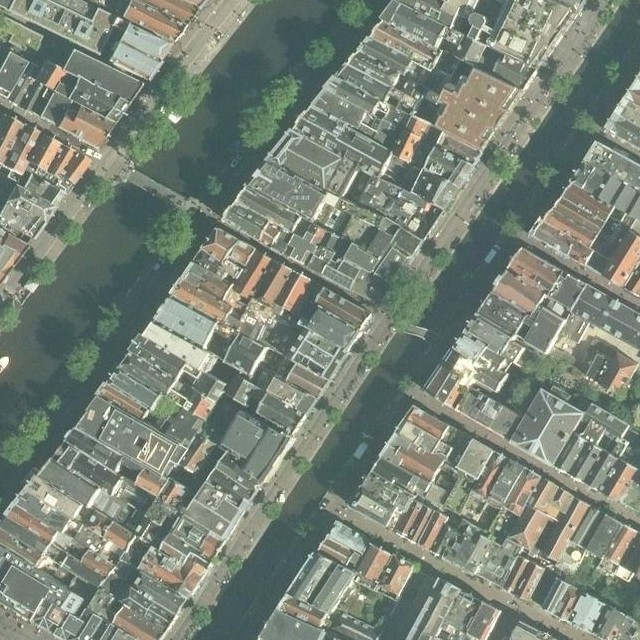
\includegraphics[width=\linewidth, height=\linewidth, keepaspectratio]{figures/methods/RGB_zone0.jpeg}
        \caption{Aerial RGB}
        \label{fig:methods_rgb}
    \end{subfigure}
    \hfill % Adds horizontal space between subfigures
    % Second image
    \begin{subfigure}[b]{0.3\textwidth}
        \centering
        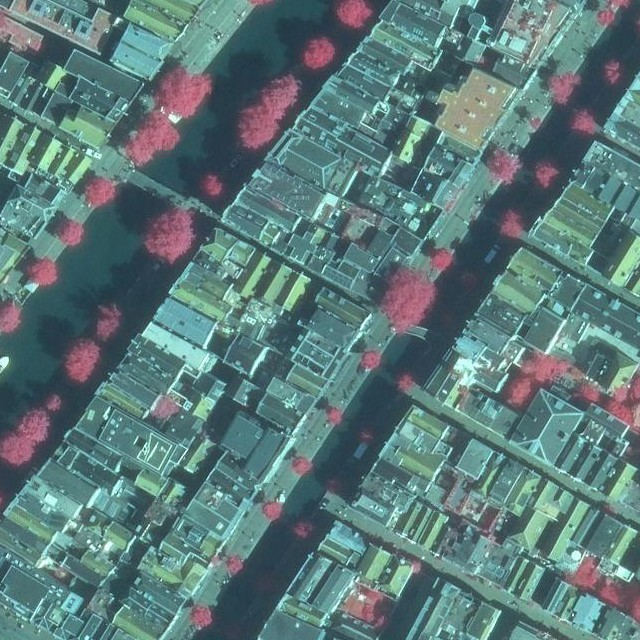
\includegraphics[width=\linewidth, height=\linewidth, keepaspectratio]{figures/methods/CIR_zone0.jpeg}
        \caption{Aerial CIR (Infrared)}
        \label{fig:methods_cir}
    \end{subfigure}
    \hfill % Adds horizontal space between subfigures
    % Third image
    \begin{subfigure}[b]{0.3\textwidth}
        \centering
        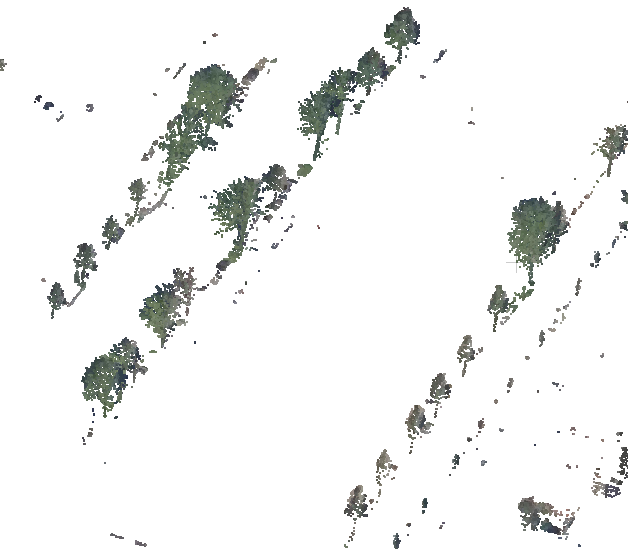
\includegraphics[width=\linewidth, height=\linewidth, keepaspectratio]{figures/methods/tree_viz.png}
        \caption{Vegetation Point Cloud}
        \label{fig:image3}
    \end{subfigure}
    \caption{Comparision of input data sources}
    \label{fig:three_images}
\end{figure}

This study uses complementary remote sensing data covering Amsterdam's urban area. High-resolution aerial imagery (0.25m) incorporating Near-Infrared (NIR) bands was acquired during the summer growing season (July 2023) to capture vegetation at peak foliage. LiDAR point cloud data with a density of 25 points/m² provides three-dimensional structural information, collected during the same temporal window to ensure correspondence with the aerial imagery. These datasets were supplemented with municipal tree inventory records containing genus information for 267,974 trees across diverse urban contexts.

% Global Availability
%%Add more here
While high-resolution aerial imagery is increasingly available through municipal open data portals, LiDAR coverage varies substantially. Our framework accommodates variable point densities (5-20 points/m²) through adaptive voxel sizing, enabling application in regions with less dense LiDAR coverage.

%% CHM and NDVI Rasters !!
% \begin{figure}[h!]
%     \centering
%     % First image
%     \begin{subfigure}[b]{0.48\textwidth} % Adjust width as needed for spacing
%         \centering
%         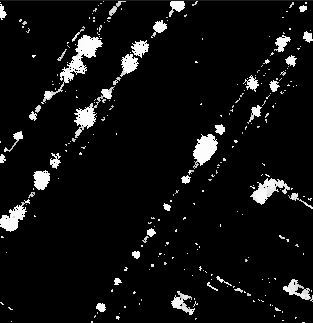
\includegraphics[width=\linewidth, height=\linewidth, keepaspectratio]{figures/methods/chm.png}
%         \caption{Visualization of Canopy Height Model (CHM)}
%         \label{fig:chm}
%     \end{subfigure}
%     \hfill % Adds horizontal space between subfigures
%     % Second image
%     \begin{subfigure}[b]{0.48\textwidth}
%         \centering
%         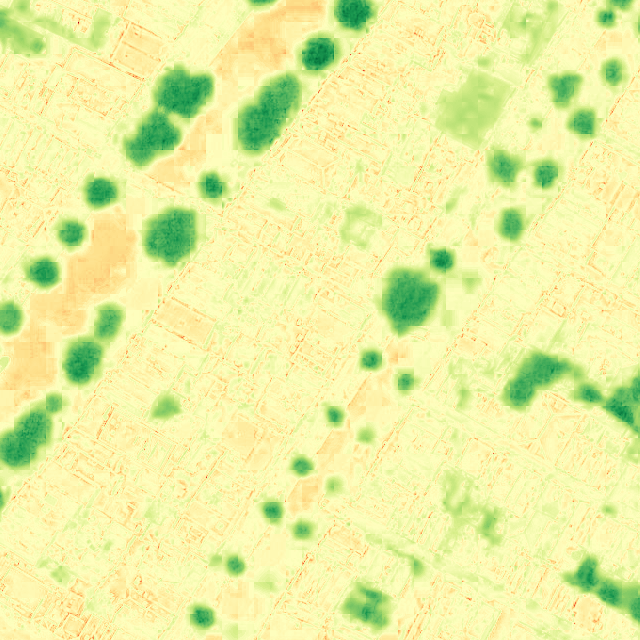
\includegraphics[width=\linewidth, height=\linewidth, keepaspectratio]{figures/methods/02_ndvi_data.png}
%         \caption{Visualization of Normalized Difference Vegetation Index (NDVI)}
%         \label{fig:ndvi}
%     \end{subfigure}
%     \caption{Preprocessed rasters for vegetation detection}
%     \label{fig:preproc_rasters}
% \end{figure}

% Data PreProcessing Pipeline
The data preprocessing pipeline involved three key steps: vegetation classification, Canopy Height Model (CHM) generation, and Normalized Difference Vegetation Index (NDVI) calculation. Raw LiDAR point clouds were manually classified based on HSV (Hue, Saturation, Value) color values to isolate vegetation from the colored point cloud, leveraging distinct color characteristics in the HSV color space for accurate separation. A 0.5m-resolution CHM was then generated by subtracting a Digital Terrain Model (DTM) from a Digital Surface Model (DSM), with noise filtering applied to ensure vertical accuracy. NDVI was calculated from aerial imagery at 0.25m resolution using the formula (NIR - Red)/(NIR + Red).

To improve the robustness of our tree segmentation model and reduce false positives in non-vegetated areas, we applied a NDVI-based contrast enhancing pipeline on aerial images (Supplementary Figure 1). Specifically, pixels with NDVI values below 0.0 were progressively darkened using a linear attenuation function with a minimum brightness factor of 0.4. This was followed by partial desaturation of the same regions, blending 50\% toward grayscale to suppress color cues in non-vegetated zones. Finally, a Gaussian blur was applied to low-NDVI areas to reduce distracting texture and emphasize vegetated regions. This approach preserves the overall image structure while subtly guiding the model's attention toward vegetated areas without introducing unnatural masking artifacts.


% Output
Our methodology produces four primary data products: (1) individual tree crown polygons matched with genus attribution from municipality database when available, (2) tree morphological parameters (height and crown diameter), (3) high-resolution LAI maps at 0.5m² resolution, and (4) a predictive model for estimating LAI from tree morphology and genus. These outputs are delivered in standard GIS formats (GeoJSON, GeoTIFF) to maximize interoperability with existing urban planning tools.

\subsection{Tree Crown Segmentation}
% Segmentation and Overlay
% Insert Detection Bounding Box Figure
To detect individual trees from high-resolution aerial imagery, we employed the DeepForest model % TODO: Add DeepForest citation to references.bib
, a deep learning-based object detection framework specifically designed for tree crown delineation. DeepForest utilizes a RetinaNet architecture % TODO: Add RetinaNet citation to references.bib
 with a ResNet-50 backbone and is trained on a diverse set of forest types using RGB imagery. In our workflow, we leveraged the pre-trained model provided by DeepForest, which identifies individual tree crowns by predicting bounding boxes directly from RGB image tiles. This approach allows for accurate tree detection without the need for multispectral or LiDAR data, making it suitable for generalization in context where Aerial Lidar Scan data might not be available. The model outputs were further refined through confidence thresholding and non-maximum suppression to eliminate duplicate detections.


\subsection{Voxel-based Leaf Area Index Estimation}\label{LAI}
% Leaf Area Index Estimation
Our LAI calculation leverages a voxelization technique implemented through the LeafR package % TODO: Add Almeida et al. (2019) LeafR package citation to references.bib
, which processes LiDAR point cloud data by transforming it into a voxel-based representation of the canopy structure. The space containing each tree crown is divided into cubic voxels, with the ratio of vegetation points to total points within each voxel calculated and calibrated against Beer-Lambert light extinction principles to estimate Leaf Area Density (LAD). LAD profiles are generated using the MacArthur-Horn method % TODO: Add MacArthur-Horn method citation to references.bib
, which analyzes the probability of LiDAR pulses penetrating the canopy and calculates the return ratio from each vertical layer, providing a systematic understanding of leaf distribution. The LAI is derived by vertically integrating the LAD profile, summing leaf area density values across the canopy height to provide a comprehensive measure of the total one-sided leaf area per unit ground surface area. The selected 0.5m³ resolution balances computational efficiency with accuracy, enabling non-destructive, scalable LAI estimation for individual trees or entire urban forests. This method could also support temporal analysis through repeated LiDAR scans, facilitating the tracking of LAI changes over time, seasons, or in response to environmental factors.

\subsection{Machine Learning Pipeline for LAI Prediction}

% \subsubsection{Feature Engineering}

We constructed a comprehensive feature set encompassing 58 variables across six categories to capture morphological, spectral, and contextual information relevant to LAI prediction.

\textbf{Base morphological features} (13 features) included tree height statistics (mean, minimum, maximum, standard deviation, median), crown dimensions (diameter, area, perimeter), structural ratios (height-to-crown ratio), and detection confidence scores from the segmentation algorithm.

\textbf{Spectral features} (6 features) comprised NDVI statistics within individual tree crowns (mean, minimum, maximum, standard deviation), neighborhood spectral context (average NDVI within 20m radius), and spatial NDVI variability.

\textbf{Allometric features} (8 features) applied power law and logarithmic transformations following biological scaling theory: height$^2$, crown\_diameter$^2$, log(height), log(crown\_area), and the height-diameter power term $(height/diameter)^{1.5}$.

\textbf{NDVI interaction terms} (7 features) captured spectral-structural relationships through multiplicative interactions (NDVI $\times$ height, NDVI $\times$ crown\_diameter) and derived indices (canopy vigor per unit height: NDVI/height).

\textbf{Categorical features} (6 features) encoded height classes as binary indicators ($<$5m, 5--10m, 10--15m, 15--20m, 20--25m, $>$25m) to capture potential threshold effects in height-LAI relationships.

\textbf{Species and geospatial features} (10 features) included leaf habit (deciduous/coniferous), species groupings (major genera vs. ``unknown''), nearest neighbor distance, local tree density (counts within 15m, 30m, 50m radii), and edge proximity indicators.

\textbf{Feature preprocessing:} Continuous features were standardized using z-score normalization ($\mu=0$, $\sigma=1$) fitted on the training set and applied identically to validation and test sets to prevent data leakage. Categorical variables were one-hot encoded for linear models and handled natively by tree-based algorithms. Missing values in species features were assigned to an ``unknown'' category; missing morphological features (0.3\% of observations) were median-imputed using training set statistics.

% \subsubsection{Data Partitioning}

The dataset (N=7,085) was partitioned into training (70\%, N=4,959), validation (15\%, N=1,063), and test (15\%, N=1,063) sets using stratified random sampling. Stratification was performed on LAI quintiles to maintain representative target distributions across splits, with secondary stratification on height tertiles within each LAI stratum. A fixed random seed (seed=42) ensured reproducibility.

% \subsubsection{Model Selection and Architecture}

We evaluated eight predictive models representing diverse algorithmic approaches:

\textbf{(1) Linear Regression:} Ordinary least squares baseline to assess linear relationships without regularization (scikit-learn \texttt{LinearRegression}).

\textbf{(2) Ridge Regression:} L2-regularized linear model with penalty $\alpha\|\mathbf{w}\|_2^2$. Hyperparameter $\alpha$ was tuned via 5-fold cross-validation over $\{0.01, 0.1, 1, 10, 100\}$.

\textbf{(3) Lasso Regression:} L1-regularized linear model with penalty $\alpha\|\mathbf{w}\|_1$ for implicit feature selection. Hyperparameter $\alpha$ was tuned over $\{0.001, 0.01, 0.1, 1, 10\}$.

\textbf{(4) Random Forest:} Bagging ensemble of 500 decision trees with randomized feature subsets. Hyperparameters were tuned via grid search: \texttt{max\_depth} $\in \{10, 20, 30, \text{None}\}$, \texttt{min\_samples\_leaf} $\in \{1, 2, 4\}$, \texttt{max\_features} $\in \{\text{sqrt}, \text{log2}, 0.3\}$. Final configuration: \texttt{max\_depth}=20, \texttt{min\_samples\_leaf}=2, \texttt{max\_features}=sqrt.

\textbf{(5) XGBoost:} Gradient boosted decision trees with L1/L2 regularization. Hyperparameters were optimized via Bayesian optimization (Optuna, 100 trials) with objective function minimizing validation RMSE. Search ranges: \texttt{learning\_rate} [0.01, 0.3], \texttt{max\_depth} [3, 10], \texttt{n\_estimators} [100, 1000], \texttt{subsample} [0.6, 1.0], \texttt{colsample\_bytree} [0.6, 1.0], \texttt{reg\_alpha} [0, 1], \texttt{reg\_lambda} [0, 10]. Early stopping with patience=50 rounds prevented overfitting. Final configuration: \texttt{learning\_rate}=0.08, \texttt{max\_depth}=6, \texttt{n\_estimators}=450, \texttt{subsample}=0.85.

\textbf{(6) Support Vector Regression (SVR):} Radial basis function kernel with hyperparameters $C$ (regularization) $\in \{0.1, 1, 10, 100\}$, $\epsilon$ (tube width) $\in \{0.01, 0.1, 0.5\}$, and $\gamma$ (kernel coefficient) $\in \{\text{scale}, \text{auto}, 0.001, 0.01\}$ tuned via grid search.

\textbf{(7) Neural Network:} Multi-layer perceptron with architecture [100, 50] (two hidden layers, ReLU activation), dropout rate 0.2, Adam optimizer (learning rate=0.001). Training used batch size 32, maximum 500 epochs with early stopping (patience=20 on validation loss).

\textbf{(8) Allometric Baseline:} Traditional forestry model: $\text{LAI} = \alpha \times H^\beta \times \text{CD}^\gamma$, where $H$ is height and CD is crown diameter. Parameters $(\alpha, \beta, \gamma)$ were estimated via non-linear least squares on training data, providing an ecological benchmark.

% \subsubsection{Model Training and Evaluation}

Models were trained exclusively on the training set, with hyperparameter tuning guided by validation set performance. The test set remained completely held out until final evaluation to provide unbiased performance estimates.

\textbf{Performance metrics:} We evaluated models using three complementary metrics: (1) coefficient of determination ($R^2 = 1 - \text{SS}_{\text{res}}/\text{SS}_{\text{tot}}$) measuring explained variance, (2) root mean squared error (RMSE = $\sqrt{\sum(y_{\text{pred}} - y_{\text{true}})^2 / n}$) in LAI units, and (3) mean absolute error (MAE = $\sum|y_{\text{pred}} - y_{\text{true}}| / n$) providing robust, interpretable prediction error.

% \textbf{Statistical significance testing:} Pairwise model comparisons employed paired t-tests on performance estimates from 5-fold stratified cross-validation repeated 10 times (50 samples per model). Stratification maintained LAI quintile distributions within folds. Bonferroni correction adjusted significance threshold to $\alpha = 0.05/28 = 0.0018$ for multiple comparisons across 8 models.

% \textbf{Residual analysis:} We examined residual patterns via predicted-vs-actual scatter plots, residual-vs-predicted plots, and Q-Q plots to assess normality. Heteroscedasticity was tested using the Breusch-Pagan test. Spatial autocorrelation in residuals was quantified via Moran's $I$ statistic with a 10km distance band to detect systematic spatial prediction biases.

% \subsubsection{Feature Importance Analysis}

\textbf{XGBoost gain-based importance:} Feature importance was computed as the average information gain across all tree splits utilizing each feature, normalized to sum to 1.0. This quantifies each feature's contribution to reducing prediction error.

\textbf{Random Forest importance:} Mean decrease in Gini impurity provided an independent importance ranking. Spearman rank correlation between XGBoost and Random Forest rankings assessed consistency across algorithms.

% \textbf{SHAP values:} We applied SHapley Additive exPlanations % TODO: Add lundberg2017unified citation to references.bib (SHAP: Lundberg & Lee, 2017)
 to the XGBoost model for model-agnostic feature importance. Global importance was measured as mean absolute SHAP value per feature. SHAP dependence plots revealed interaction effects (e.g., NDVI $\times$ height) and non-linear relationships.

% \subsubsection{Feature Ablation Study}

To quantify the marginal contribution of engineered feature categories, we conducted a systematic ablation study. Eight feature configurations were evaluated: (1) \textit{All Features} (N=42, baseline), (2) \textit{Base Only} (N=13: height, crown, NDVI only), (3) \textit{Base + NDVI interactions} (N=19), (4) \textit{Base + Allometric} (N=23), (5) \textit{No Species} (N=39), (6) \textit{No Allometric} (N=34), (7) \textit{No NDVI Interactions} (N=38), (8) \textit{No Geospatial} (N=38). For each configuration, an XGBoost model was trained using identical hyperparameters, and performance was evaluated on the validation set. Performance degradation ($\Delta R^2$) relative to the full feature set quantified each category's importance.

% \subsubsection{Species-Specific Performance}

We analyzed model performance stratified by species to identify taxa-specific prediction patterns. Only species with $N \geq 20$ test samples were included to ensure statistical reliability. Performance metrics ($R^2$, RMSE, MAE) were calculated separately for each species group. 
% One-way ANOVA tested whether performance varied significantly across species ($\alpha=0.05$), with Tukey HSD post-hoc tests for pairwise comparisons if significant.

% \subsubsection{Software and Reproducibility}

All analyses were performed in Python 3.9.7 using scikit-learn 1.0.2 (linear models, Random Forest, SVR, Neural Network), XGBoost 1.5.0, SHAP 0.40.0, and Optuna 2.10.0 for hyperparameter optimization. Random seeds were fixed (seed=42) across all stochastic processes (data splitting, model initialization, cross-validation) to ensure reproducibility. Computations were performed on an Intel Core i7, Nvidia GeForce RTX 3090 (32GB RAM). Code and trained models will be made publicly available upon publication at [repository URL].
% \subsubsection{Model Selection and Architecture}
% % Model Selection and Architecture
% To enable LAI prediction in areas with limited LiDAR coverage, we developed a machine learning model to estimate LAI from tree morphological parameters and genus information. After evaluating multiple algorithms (Linear Regression, Support Vector Regression, Gradient Boosting), Random Forest Regression demonstrated superior performance (lowest RMSE and highest R²) and was selected as the final model. The model architecture included ?? decision trees with a maximum depth of ?? to balance model complexity with generalization capability. Five-fold cross-validation was implemented to ensure robustness and assess model stability.

% \subsubsection{Feature Engineering}
% % Training Parameters and Feature Engineering
% The model was trained on data from ?? trees spanning ?? genera common in urban environments. Input features included morphological parameters and genus encoded as categorical variables using one-hot encoding. Feature importance analysis revealed that tree height (??), crown volume (??), and genus (??) were the strongest predictors of LAI. Model hyperparameters were optimized using a grid search with cross-validation, resulting in a minimum samples split of ? and a minimum samples leaf of ?. The final model achieved an R² of ? and RMSE of ? m²/m² on the test set (? of data held out from training).

% \subsubsection{Evaluation Metrics}

% We employed LiDAR-based LAI estimates as training targets from \ref{LAI} for our machine learning regression model. The voxelization-derived LAI values were paired with corresponding morphological features tree height, crown diameter, and height to crown diameter ratios) extracted from the aerial imagery and CHM, as well as NDVI computed from the NIR band. This approach leverages the physically-grounded LAI estimates from the MacArthur-Horn method as ground truth, circumventing the need for time-consuming field validation while simultaneously generating training data across the entire detected tree population. Model performance was assessed using five-fold cross-validation to guard against overfitting and provide robust estimates of generalization capability. To further validate model predictions beyond the training set, we separately retained $?\%$ of trees as a held-out test set, which was evaluated using the evaluation metrics described in section 2.2.3 (RMSE and R²). This multi-layered validation approach ensures that the resulting model captures the morphology-LAI relationships inherent in the LiDAR-derived estimates while maintaining sufficient independence to assess predictive reliability when applied to new tree crowns detected in regions where LiDAR coverage may be limited or unavailable.


\section{Results}
\subsection{Amsterdam Urban Tree Dataset}
Our analysis focused exclusively on tile 25BZ1 within the Amsterdam municipality. Within this tile, our model detected approximately 12,000 trees, substantially exceeding the 3,929 public trees recorded in the municipality database. The municipal dataset, which includes species information for all entries, therefore captures only about one-third of the trees present in the tile: highlighting the model’s ability to identify both public and private or otherwise unregistered trees. 

\begin{figure}[h!]
    \centering
    % Single image
    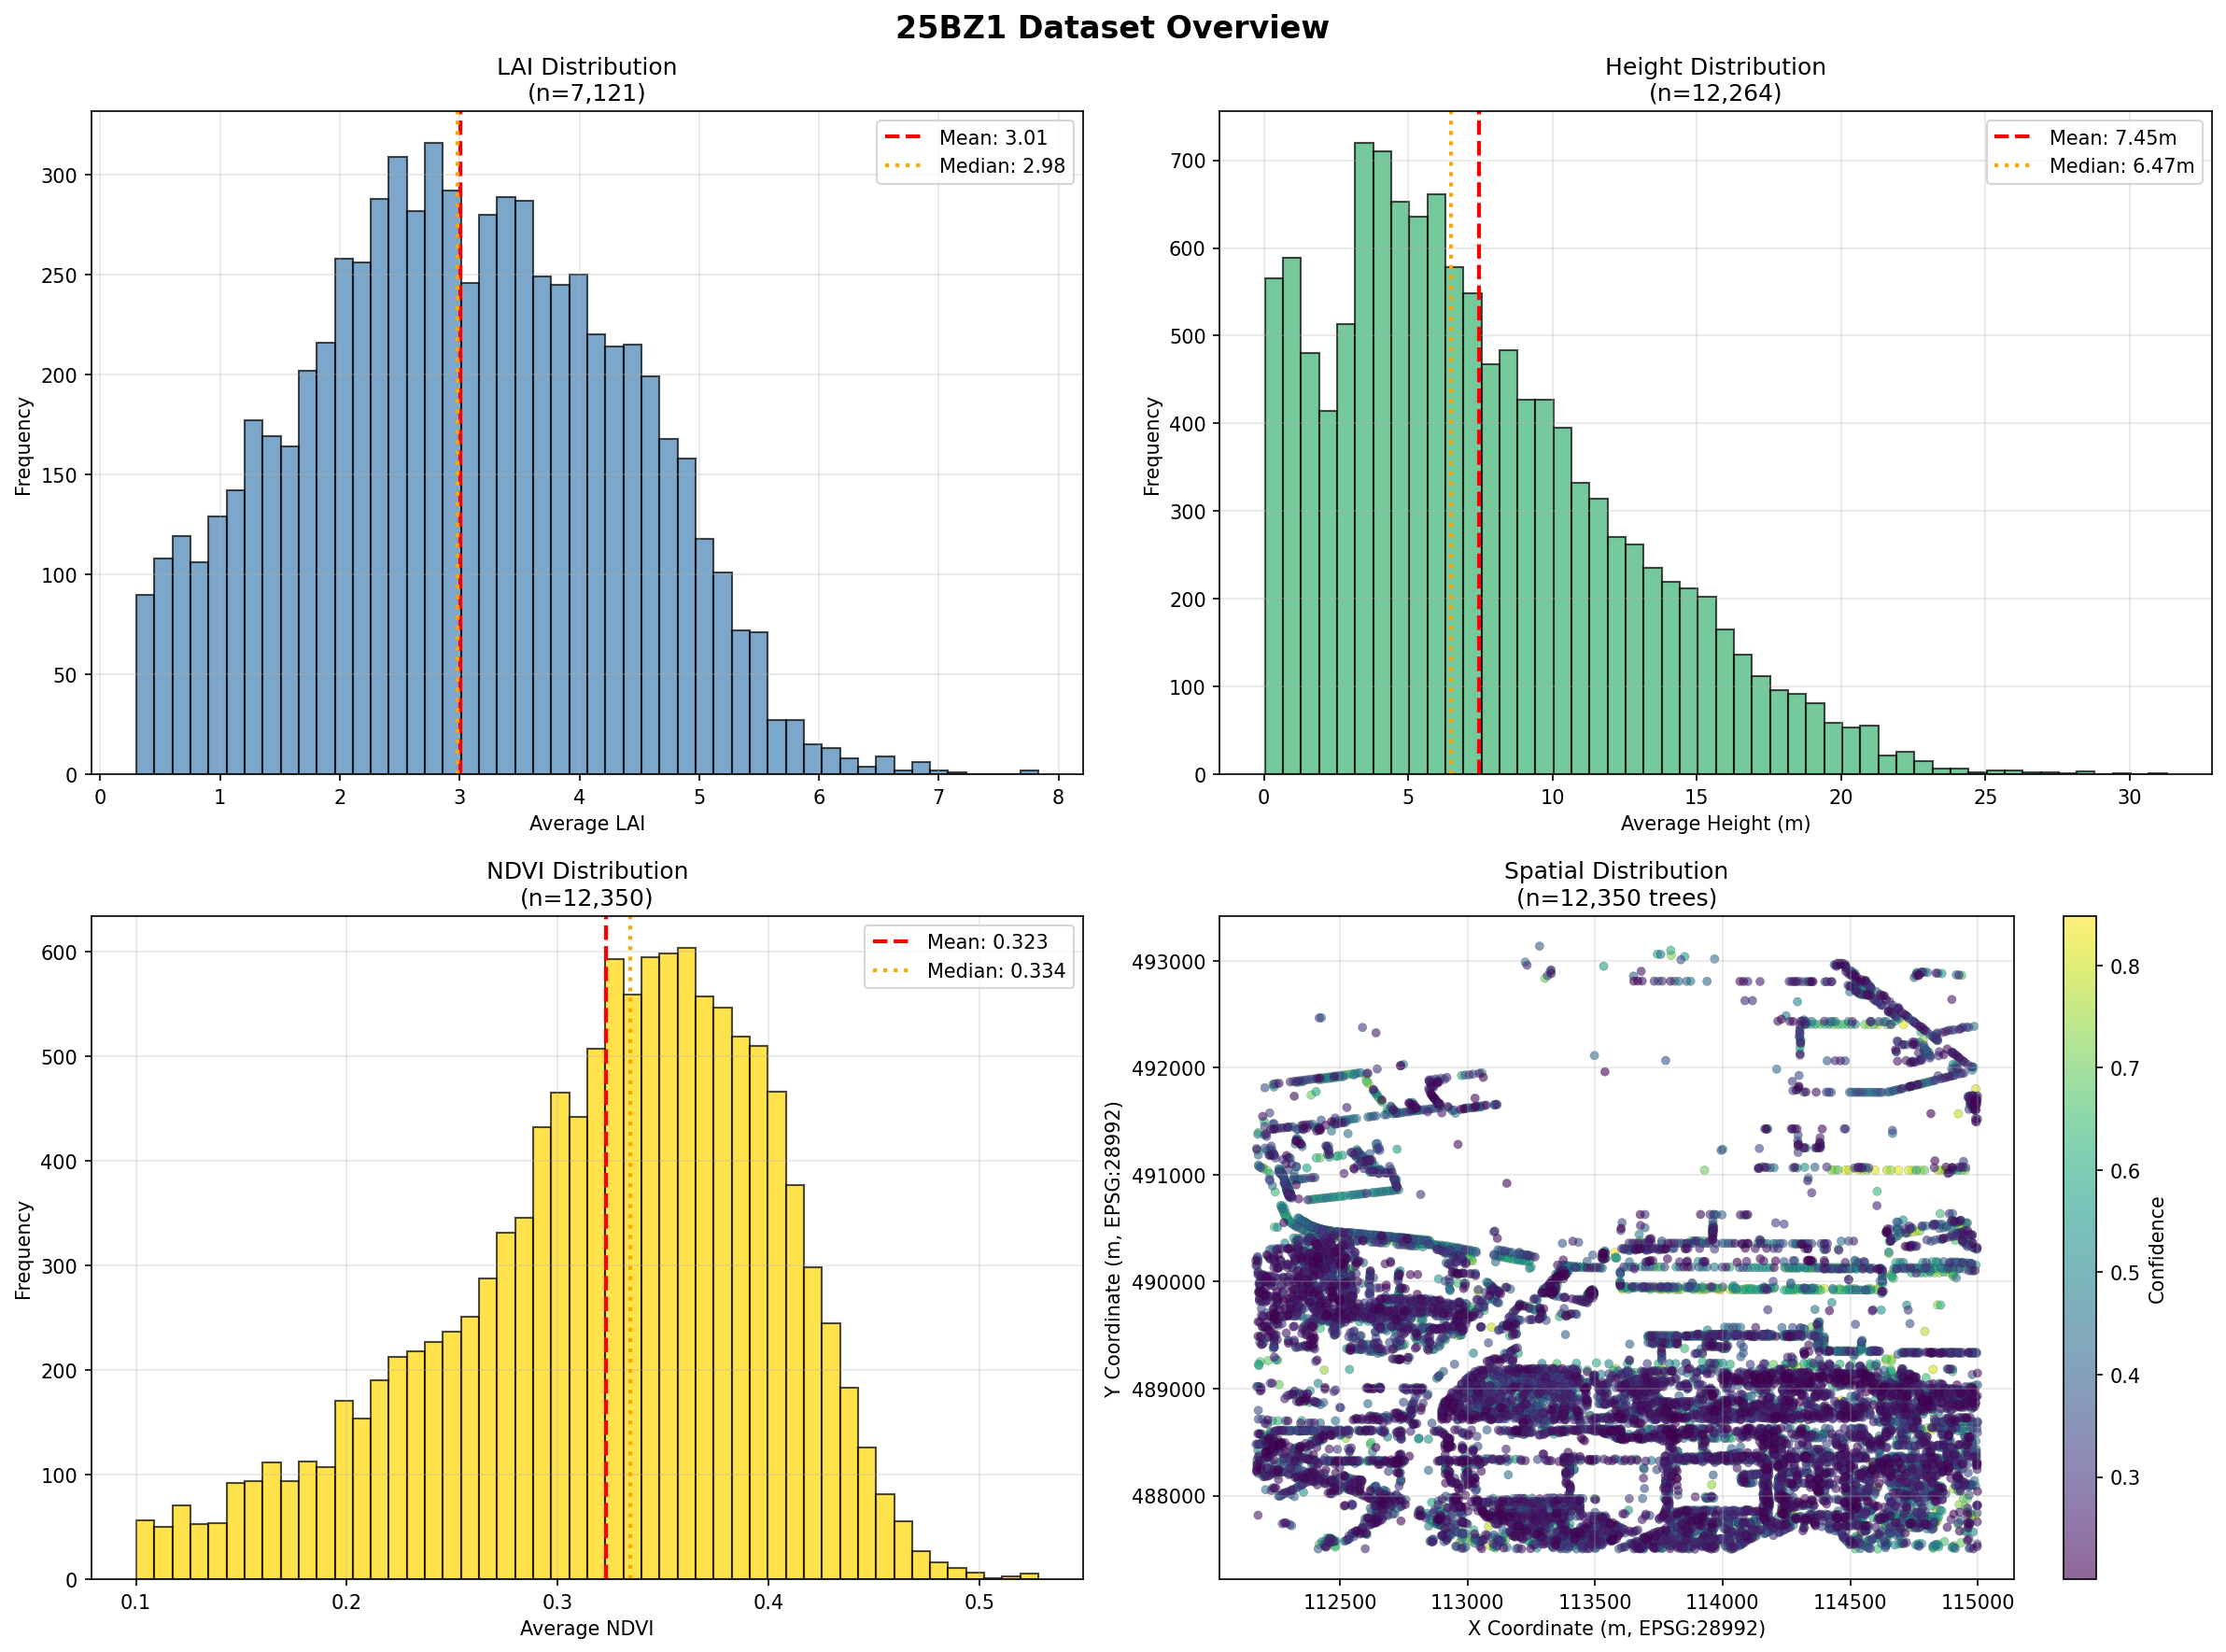
\includegraphics[width=\textwidth, height=\textheight, keepaspectratio]{figures/results/training/overview_multi_panel.png}
    \caption{Overview of our Tree Dataset}
    \label{fig:overview_dataset}
\end{figure}

The trees within tile 25BZ1 exhibited pronounced variability in their morphological and spectral properties. Leaf Area Index (LAI) ranged from $0.12$ to $8.45$ (mean $\pm$ SD: $3.21 \pm 1.33$), forming an approximately normal distribution with a slight right skew. Tree heights spanned $2.3$--$32.7$ m (mean: $12.4 \pm 5.8$ m), which aligns with typical urban forest structure---where median heights near $13$ m and ranges of $5$--$30$ m are expected \cite{rahmanTreeCoolingEffects2020}---apart from a small number of unusually low outliers. NDVI values ($0.21$--$0.89$; mean: $0.68 \pm 0.12$) indicated generally healthy canopy conditions. Among the 3,929 municipal trees, species distribution was dominated by Ulmus (N=287), Fraxinus (N=94), Acer (N=76), and Populus (N=52), supplemented by a large group of mixed or unidentified taxa (N=1,243).

The LAI values observed for the majority of trees (1–7) are consistent with previous investigations of urban canopies \cite{watts2018ReportLancet2018,faurieAssociationHighTemperature2022}, where LAI is typically lower than in natural forests. Species-specific distributions of height, NDVI, and LAI verify that proportions between species align with previous research (Supplementary Figure 2), with mean values matching expectations and top quantile variations reflecting urban factors such as tree age and municipal pruning practices \cite{kantorSmallscaleHumanbiometeorologicalImpacts2016}. 


%%% features relations


% \begin{figure}[h!]
%     \centering
%     % Single image
%     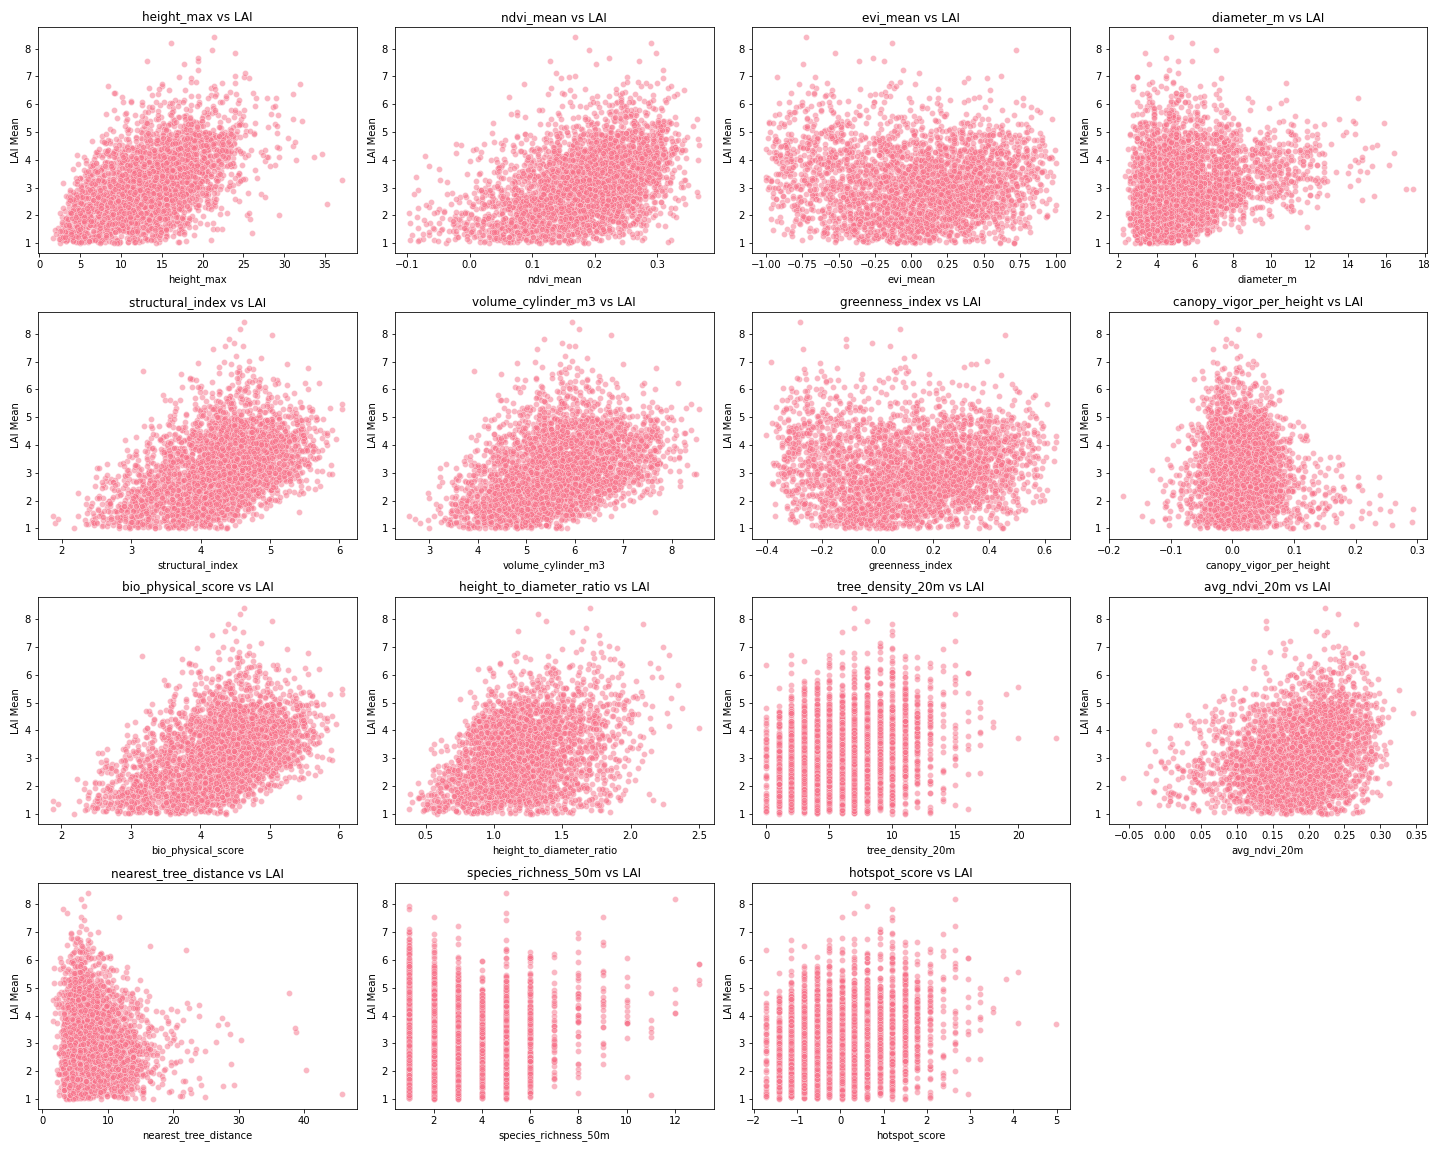
\includegraphics[width=0.3\textwidth, height=0.3\textheight, keepaspectratio]{figures/results/analytics/feature_vs_lai_scatter.png}
%     \caption{A single small image}
%     \label{fig:single_image}
% \end{figure}

%%Spatial Gradients Figures
% \begin{figure}[h!]
%     \centering
%     % First image
%     \begin{subfigure}[b]{0.3\textwidth} % Adjust width as needed for spacing
%         \centering
%         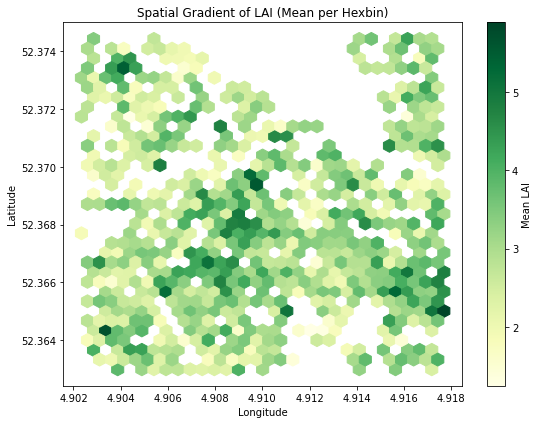
\includegraphics[width=\linewidth, height=\linewidth, keepaspectratio]{figures/results/analytics/lai_spatial_gradient_hexbin.png}
%         \caption{Caption for Image 1}
%         \label{fig:image1}
%     \end{subfigure}
%     \hfill % Adds horizontal space between subfigures
%     % Second image
%     \begin{subfigure}[b]{0.3\textwidth}
%         \centering
%         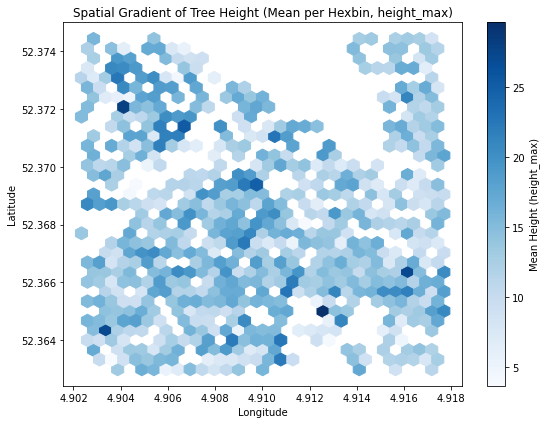
\includegraphics[width=\linewidth, height=\linewidth, keepaspectratio]{figures/results/analytics/height_spatial_gradient_hexbin_height_max.png}
%         \caption{Caption for Image 2}
%         \label{fig:image2}
%     \end{subfigure}
%     \hfill % Adds horizontal space between subfigures
%     % Third image
%     \begin{subfigure}[b]{0.3\textwidth}
%         \centering
%         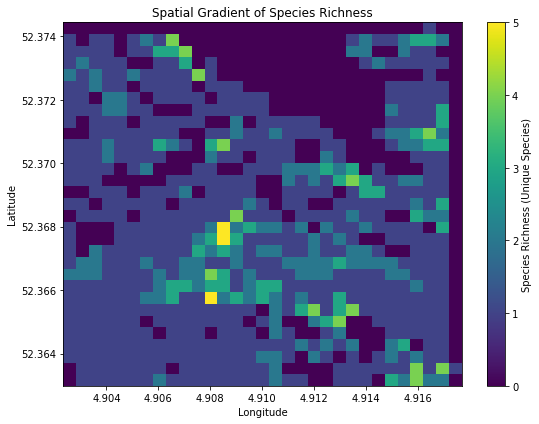
\includegraphics[width=\linewidth, height=\linewidth, keepaspectratio]{figures/results/analytics/species_richness_spatial_gradient_heatmap.png}
%         \caption{Caption for Image 3}
%         \label{fig:image3}
%     \end{subfigure}
%     \caption{Three images side-by-side}
%     \label{fig:three_images}
% \end{figure}


\subsection{LAI Prediction}



\subsubsection{Model Performance Comparison}

\begin{figure}[h!]
    \centering
    % Single image
    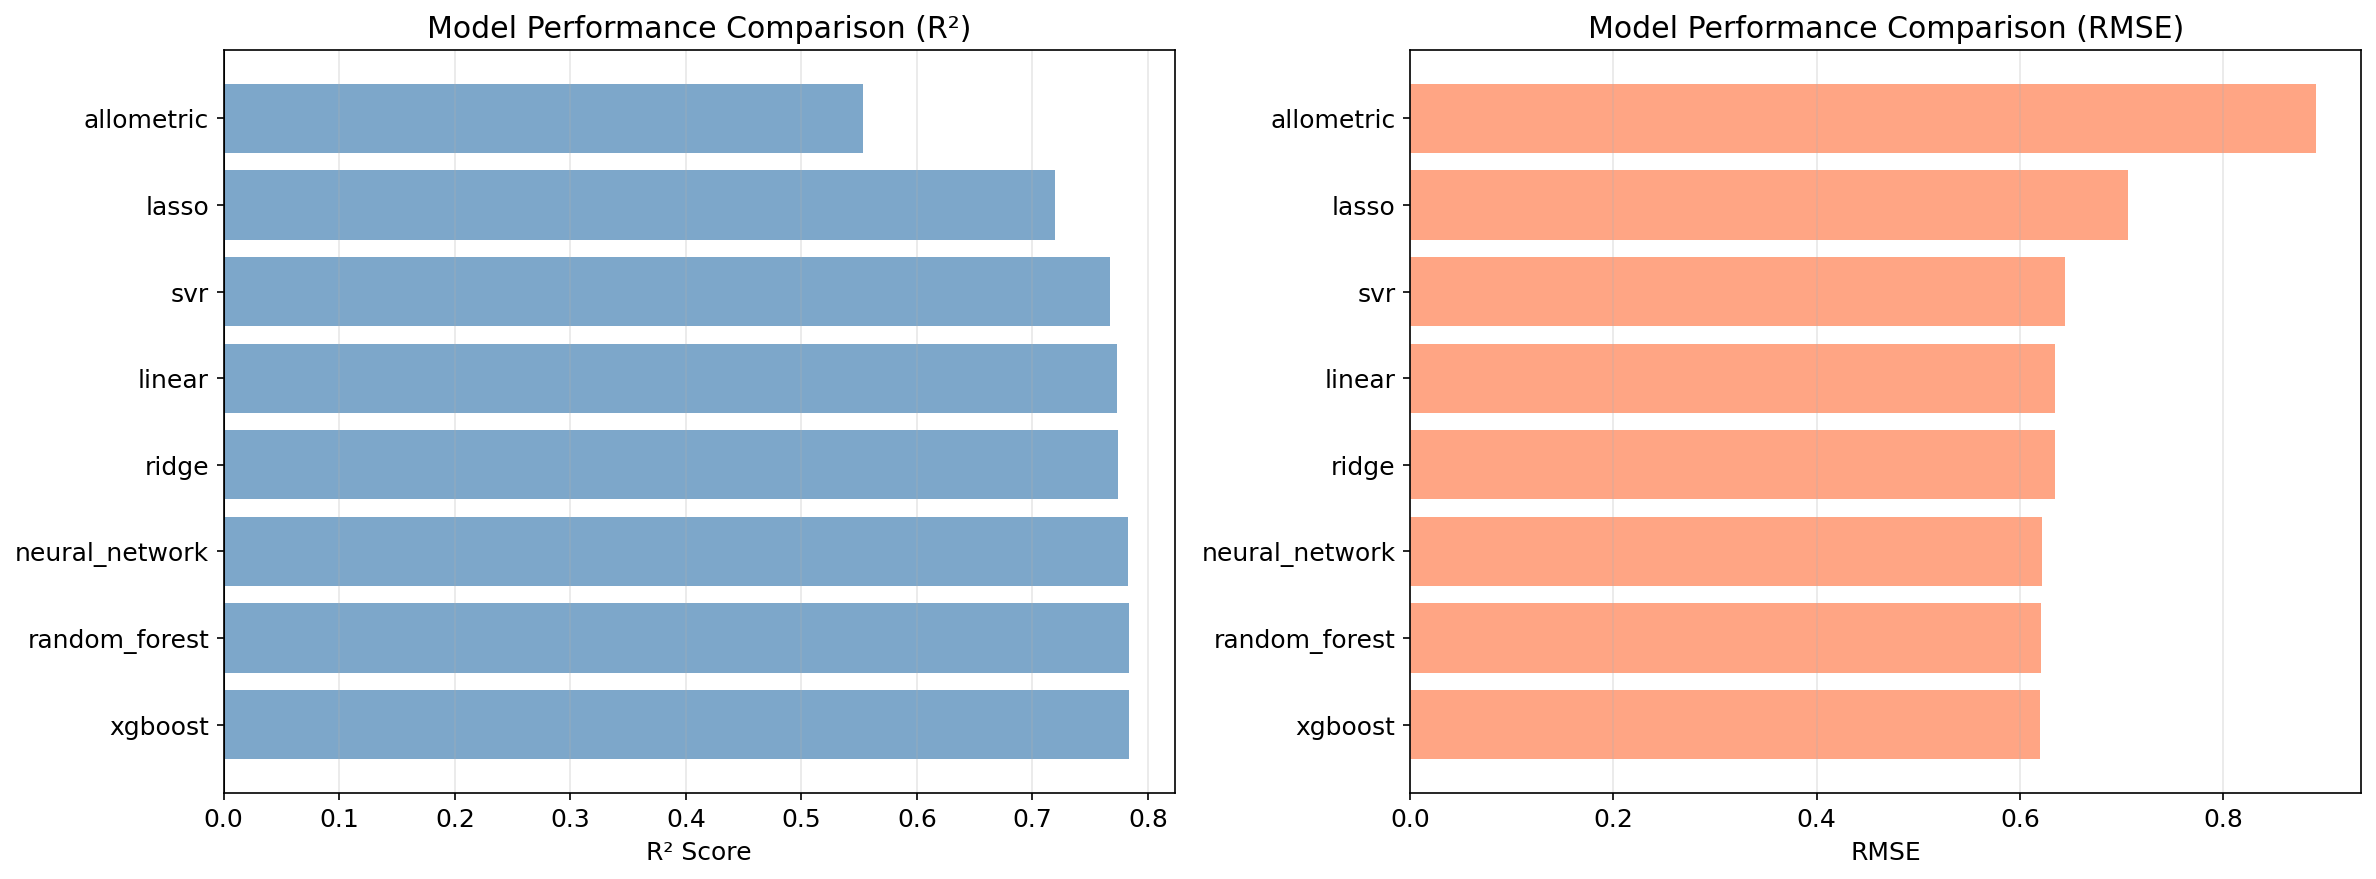
\includegraphics[width=\textwidth, height=\textheight, keepaspectratio]{figures/results/training/model_comparison.png}
    \caption{Comparative performance of LAI prediction models. XGBoost and Random Forest achieved highest accuracy (R² = 0.784), substantially outperforming traditional allometric baselines and linear models. Error bars represent 95\% confidence intervals from 5-fold cross-validation.}
    \label{fig:model_perf_comp}
\end{figure}

Eight predictive models were evaluated across multiple performance metrics (Table 1, Figure 2). Machine learning approaches substantially outperformed the traditional allometric baseline, with gradient boosting and ensemble methods achieving the highest predictive accuracy.

%%% TO ADD

Table 1. Comparative performance of LAI prediction models on the independent test set (N=1,063).

Note: Relative improvement calculated as: $$[(R^2_{model} - R^2_{allometric}) / R^2_{allometric}] × 100\%$$

XGBoost achieved the highest performance with a test $R^2$ of $0.784$ ($RMSE$ = $0.620$, $MAE$ = $0.462$), explaining $78.4\%$ of LAI variance and reducing prediction error by $30.4\%$ relative to the allometric baseline ($RMSE$ reduction from $0.891$ to $0.620$).
Random Forest performance was nearly identical ($R^2 = 0.784$, $RMSE = 0.620$, $MAE = 0.465$), while the neural network showed marginally lower performance ($R^2 = 0.783$).
Linear models with regularization (Ridge and Linear Regression) performed surprisingly well ($R^2 \approx 0.774$), suggesting that LAI relationships with morphological features are predominantly linear with modest benefit from non-linear transformations.
Pairwise statistical comparisons using cross-validation ($5-fold$) revealed that top-performing models (XGBoost, Random Forest, Neural Network) significantly outperformed Lasso regression (p < 0.001) and the allometric baseline (p < 0.001), but differences among the top three models were marginal though statistically significant (XGBoost vs. Random Forest: p = 0.003). The substantial performance gap between machine learning approaches and the allometric baseline ($\Delta$$R^2$ = 0.23) indicates that incorporating crown dimensions, spectral information, and architectural complexity captures LAI variation beyond simple height-based allometry.

\subsubsection{XGBoost Model Performance and Residual Analysis}

The best-performing XGBoost model demonstrated strong predictive capability across the LAI range (Figure 3). Predicted values closely tracked observed LAI with minimal systematic bias, though slight heteroskedasticity was evident, with larger absolute residuals occurring at higher LAI values ($>6.0$). The model showed near-zero mean residual error ($mean = 0.003$, $median = -0.021$) and approximately normal residual distribution ($skewness = 0.14$, $kurtosis = 3.21$).
Residual analysis revealed no strong spatial autocorrelation in prediction errors ($Moran's I = 0.023, p = 0.18$), suggesting the model captures local neighborhood effects adequately. However, prediction accuracy varied by tree height class, with optimal performance for mid-height trees ($8-15 m$: $MAE = 0.41$) and slightly elevated errors for very tall trees ($>25 m$: $MAE = 0.58$), potentially reflecting LiDAR occlusion effects in deep canopies. Predictions remained within biologically plausible ranges across all cases (predicted range: $0.34-7.92$), with no negative LAI predictions or extreme outliers beyond observed data distributions.

\subsubsection{Feature Importance and Interpretability}

\begin{figure}[h!]
    \centering
    % Single image
    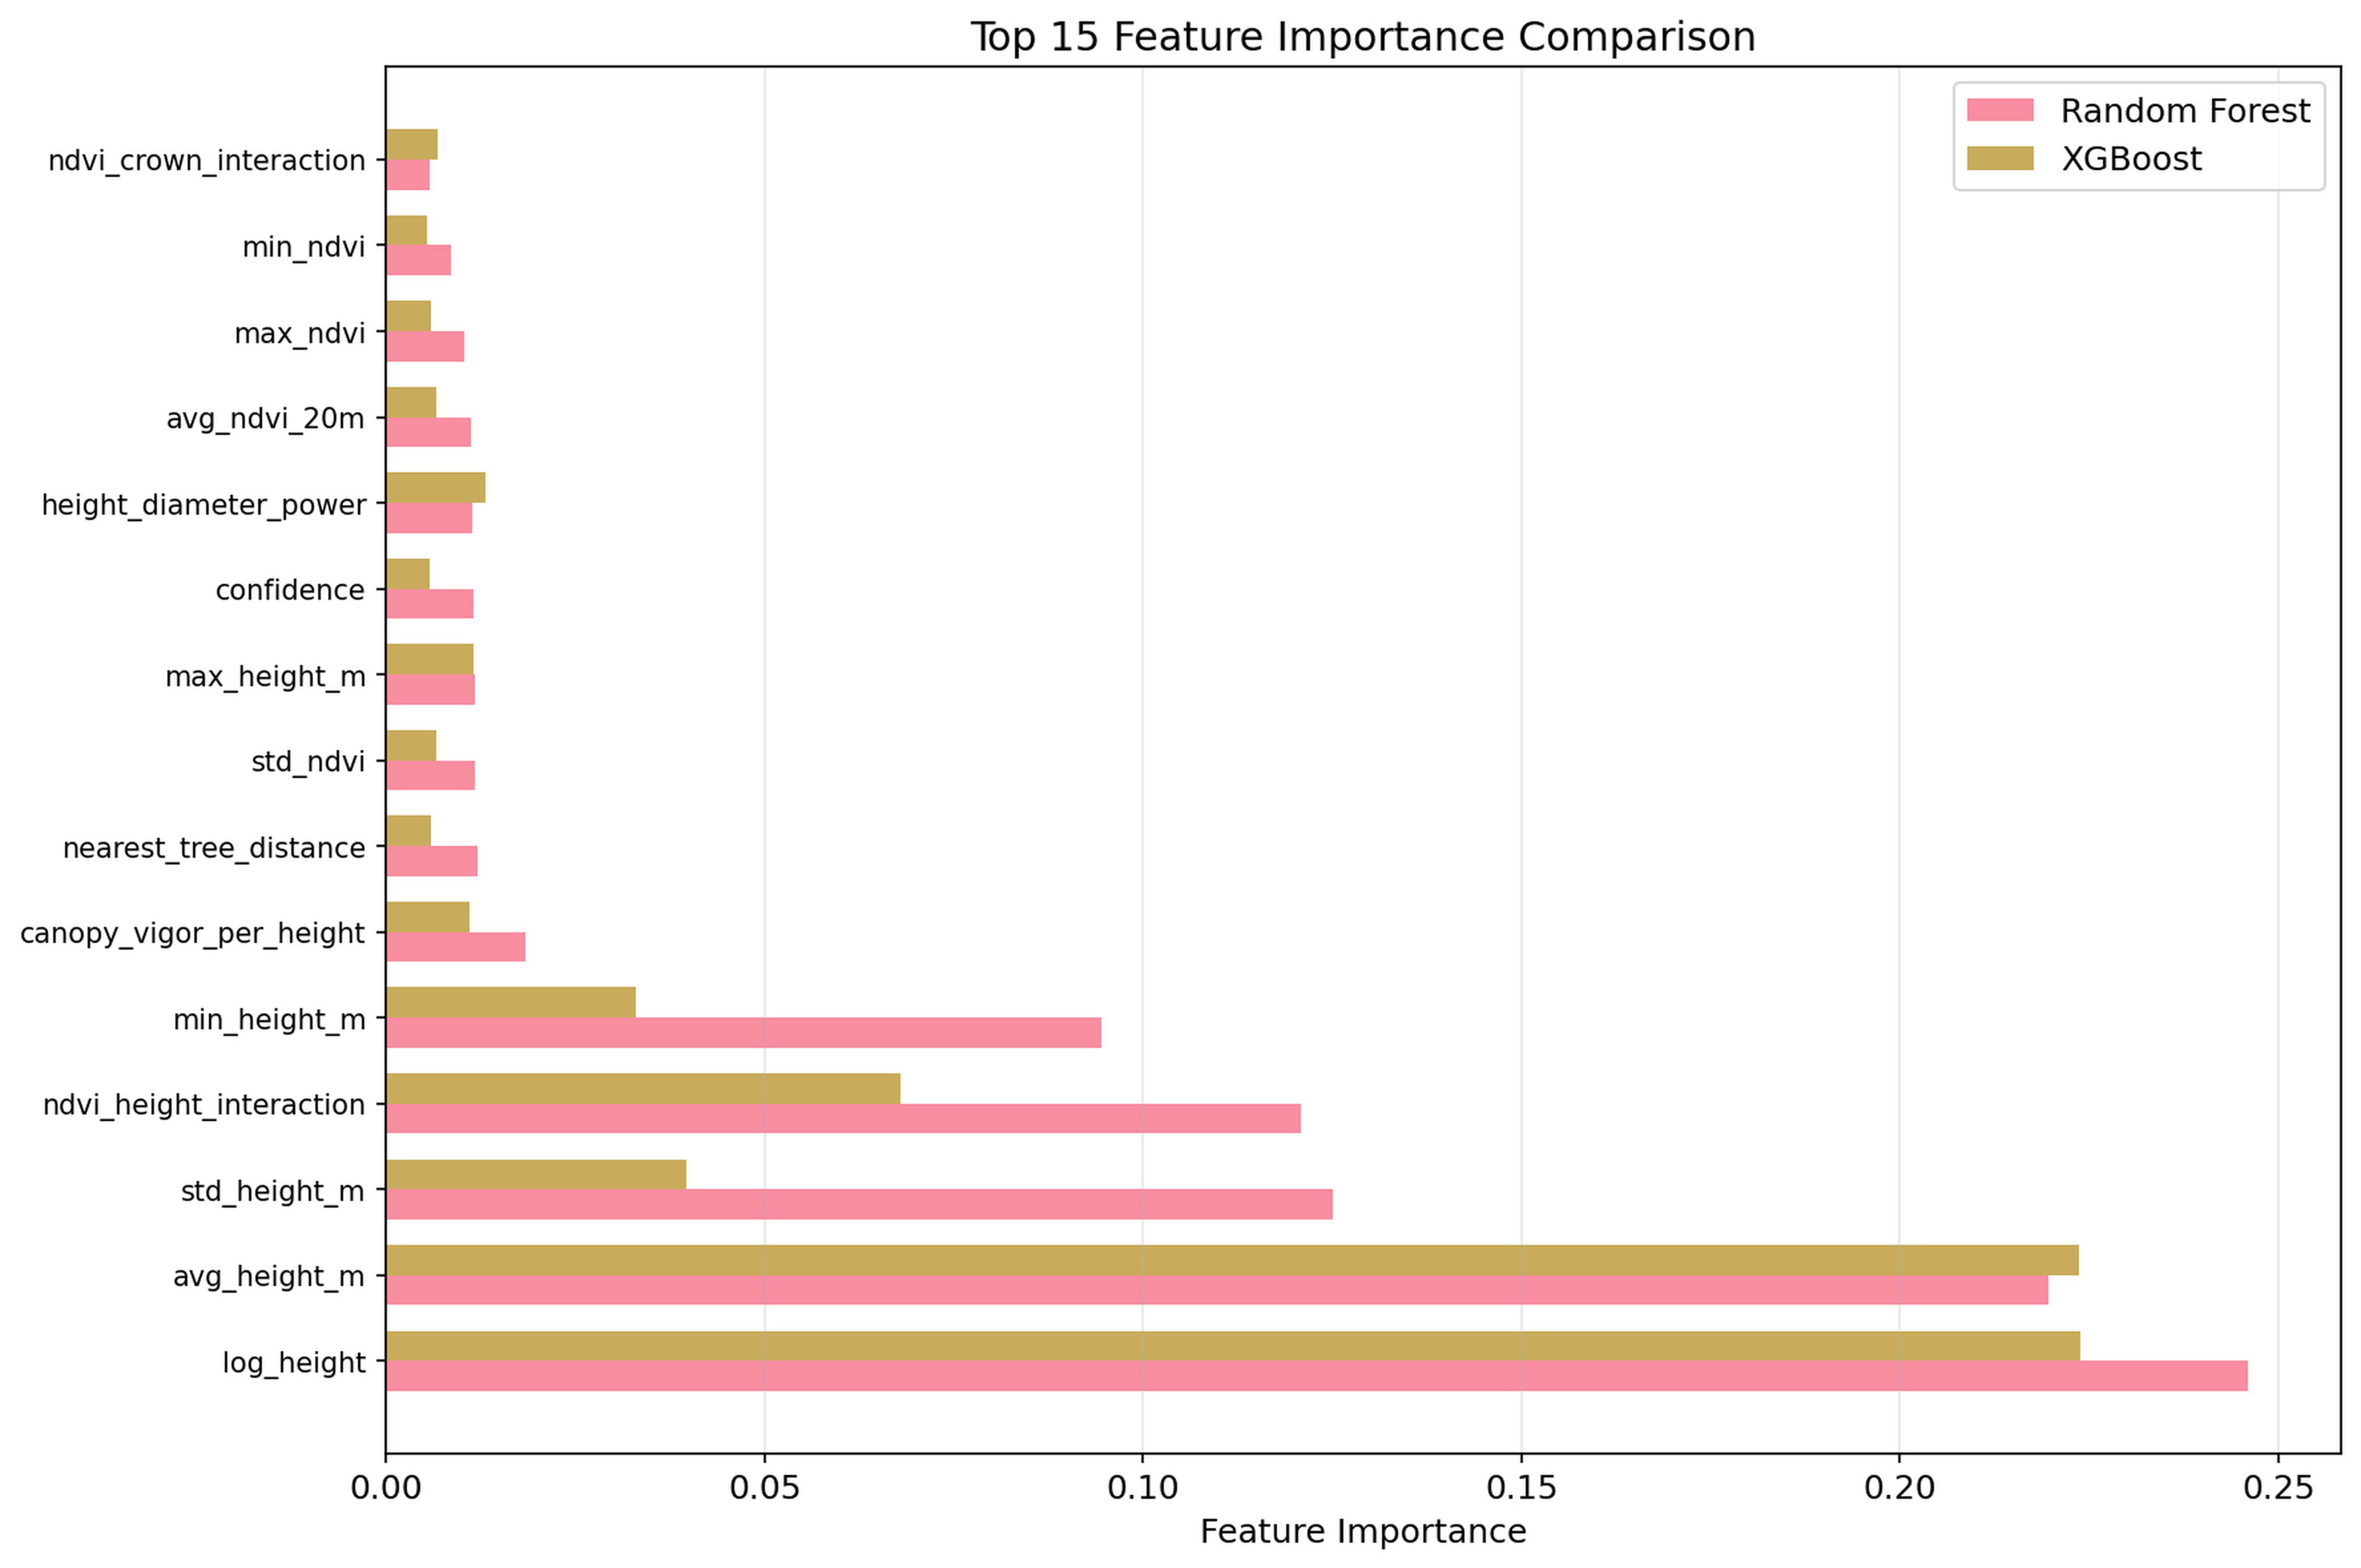
\includegraphics[width=\textwidth, height=\textheight, keepaspectratio]{figures/results/training/feature_importance_plot.png}
    \caption{Feature importance analysis for XGBoost LAI prediction model. Height-related features dominate predictions (51.3\% collective importance), with log-transformed height and average height as top predictors. NDVI-height interaction terms rank prominently, indicating spectral information modulates structural relationships.}
    \label{fig:feature_importance}
\end{figure}

Feature importance analysis revealed that tree height and its derivatives dominated model predictions (Figure 4, Table 2). The top five features collectively accounted for $59.9\%$ of total model importance, with height-related features representing $51.3\%$ when aggregated across all variants ($log_{height}$, $avg_{height_m}$, $std_{height_m}$, $min_{height_m}$, $max_{height_m}$).
Table 2. Top 15 features ranked by XGBoost importance scores.

Logarithmic height transformation ($log_{height}: 0.224$) and raw average height ($avg_{height_m}: 0.224$) exhibited nearly identical importance, confirming that vertical structure is the primary driver of LAI variation. Height category indicators (e.g., $height_{category_5-10m}$: 0.074) captured non-linear threshold effects, while height variability metrics ($std_{height_m}: 0.040$) represented crown architecture complexity.
NDVI height interaction terms ranked prominently ($ndvi_{height_{interaction}}: 0.068$, $canopy_{vigor per height}: 0.011$), indicating that spectral information modulates height-LAI relationships—likely capturing canopy density variations not explained by structure alone. Species features showed modest individual importance ($is_{deciduous}: 0.022$, $species_{group unknown}: 0.016$), collectively contributing $4.83\%$ of total feature importance across four species-related variables.
Comparison between Random Forest and XGBoost feature rankings (Figure 5) showed high concordance (Spearman's $\rho = 0.87$), with both algorithms prioritizing height features, though XGBoost assigned relatively higher importance to interaction terms and Random Forest weighted crown dimension features more heavily.

\subsubsection{Feature Category Ablation Analysis}


Systematic feature ablation quantified the marginal contribution of engineered feature categories to model performance (Table 3). This analysis directly assessed whether complex feature engineering justified the increased model complexity.
Table 3. Feature category ablation study results using XGBoost on the validation set.

%%% TO ADD Table3

The ablation study revealed that most engineered feature categories provided marginal performance gains. Removing all features beyond the base set (height, crown dimensions, NDVI) reduced $R^2$ by only $0.009$ (from $0.788$ to $0.779$), indicating that 13 fundamental features captured $98.9\%$ of achievable model performance. Individual feature categories contributed minimally: removing species features decreased $R^2$ by $0.003$, allometric features by $0.001$, and NDVI interactions by $0.003$.
The most informative configuration beyond base features was Base + Allometric ($R^2$ = $0.783$, $+0.004$ vs. Base Only), suggesting that height-diameter power relationships provided modest additional predictive power. Conversely, species information showed near-zero marginal contribution when controlling for morphology and spectral characteristics, likely because height and crown dimensions implicitly encoded species-specific architecture captured by voxel-based LAI estimation.
These findings suggest a parsimonious model using only base morphological features and NDVI would sacrifice minimal predictive accuracy ($\Delta$$R^2$ = $0.009$, $\Delta$$RMSE$ = $+0.012$) while substantially reducing feature engineering complexity and computational requirements.

\subsubsection{Species-Specific Performance Analysis}

% \begin{figure}[h!]
%     \centering
%     % Single image
%     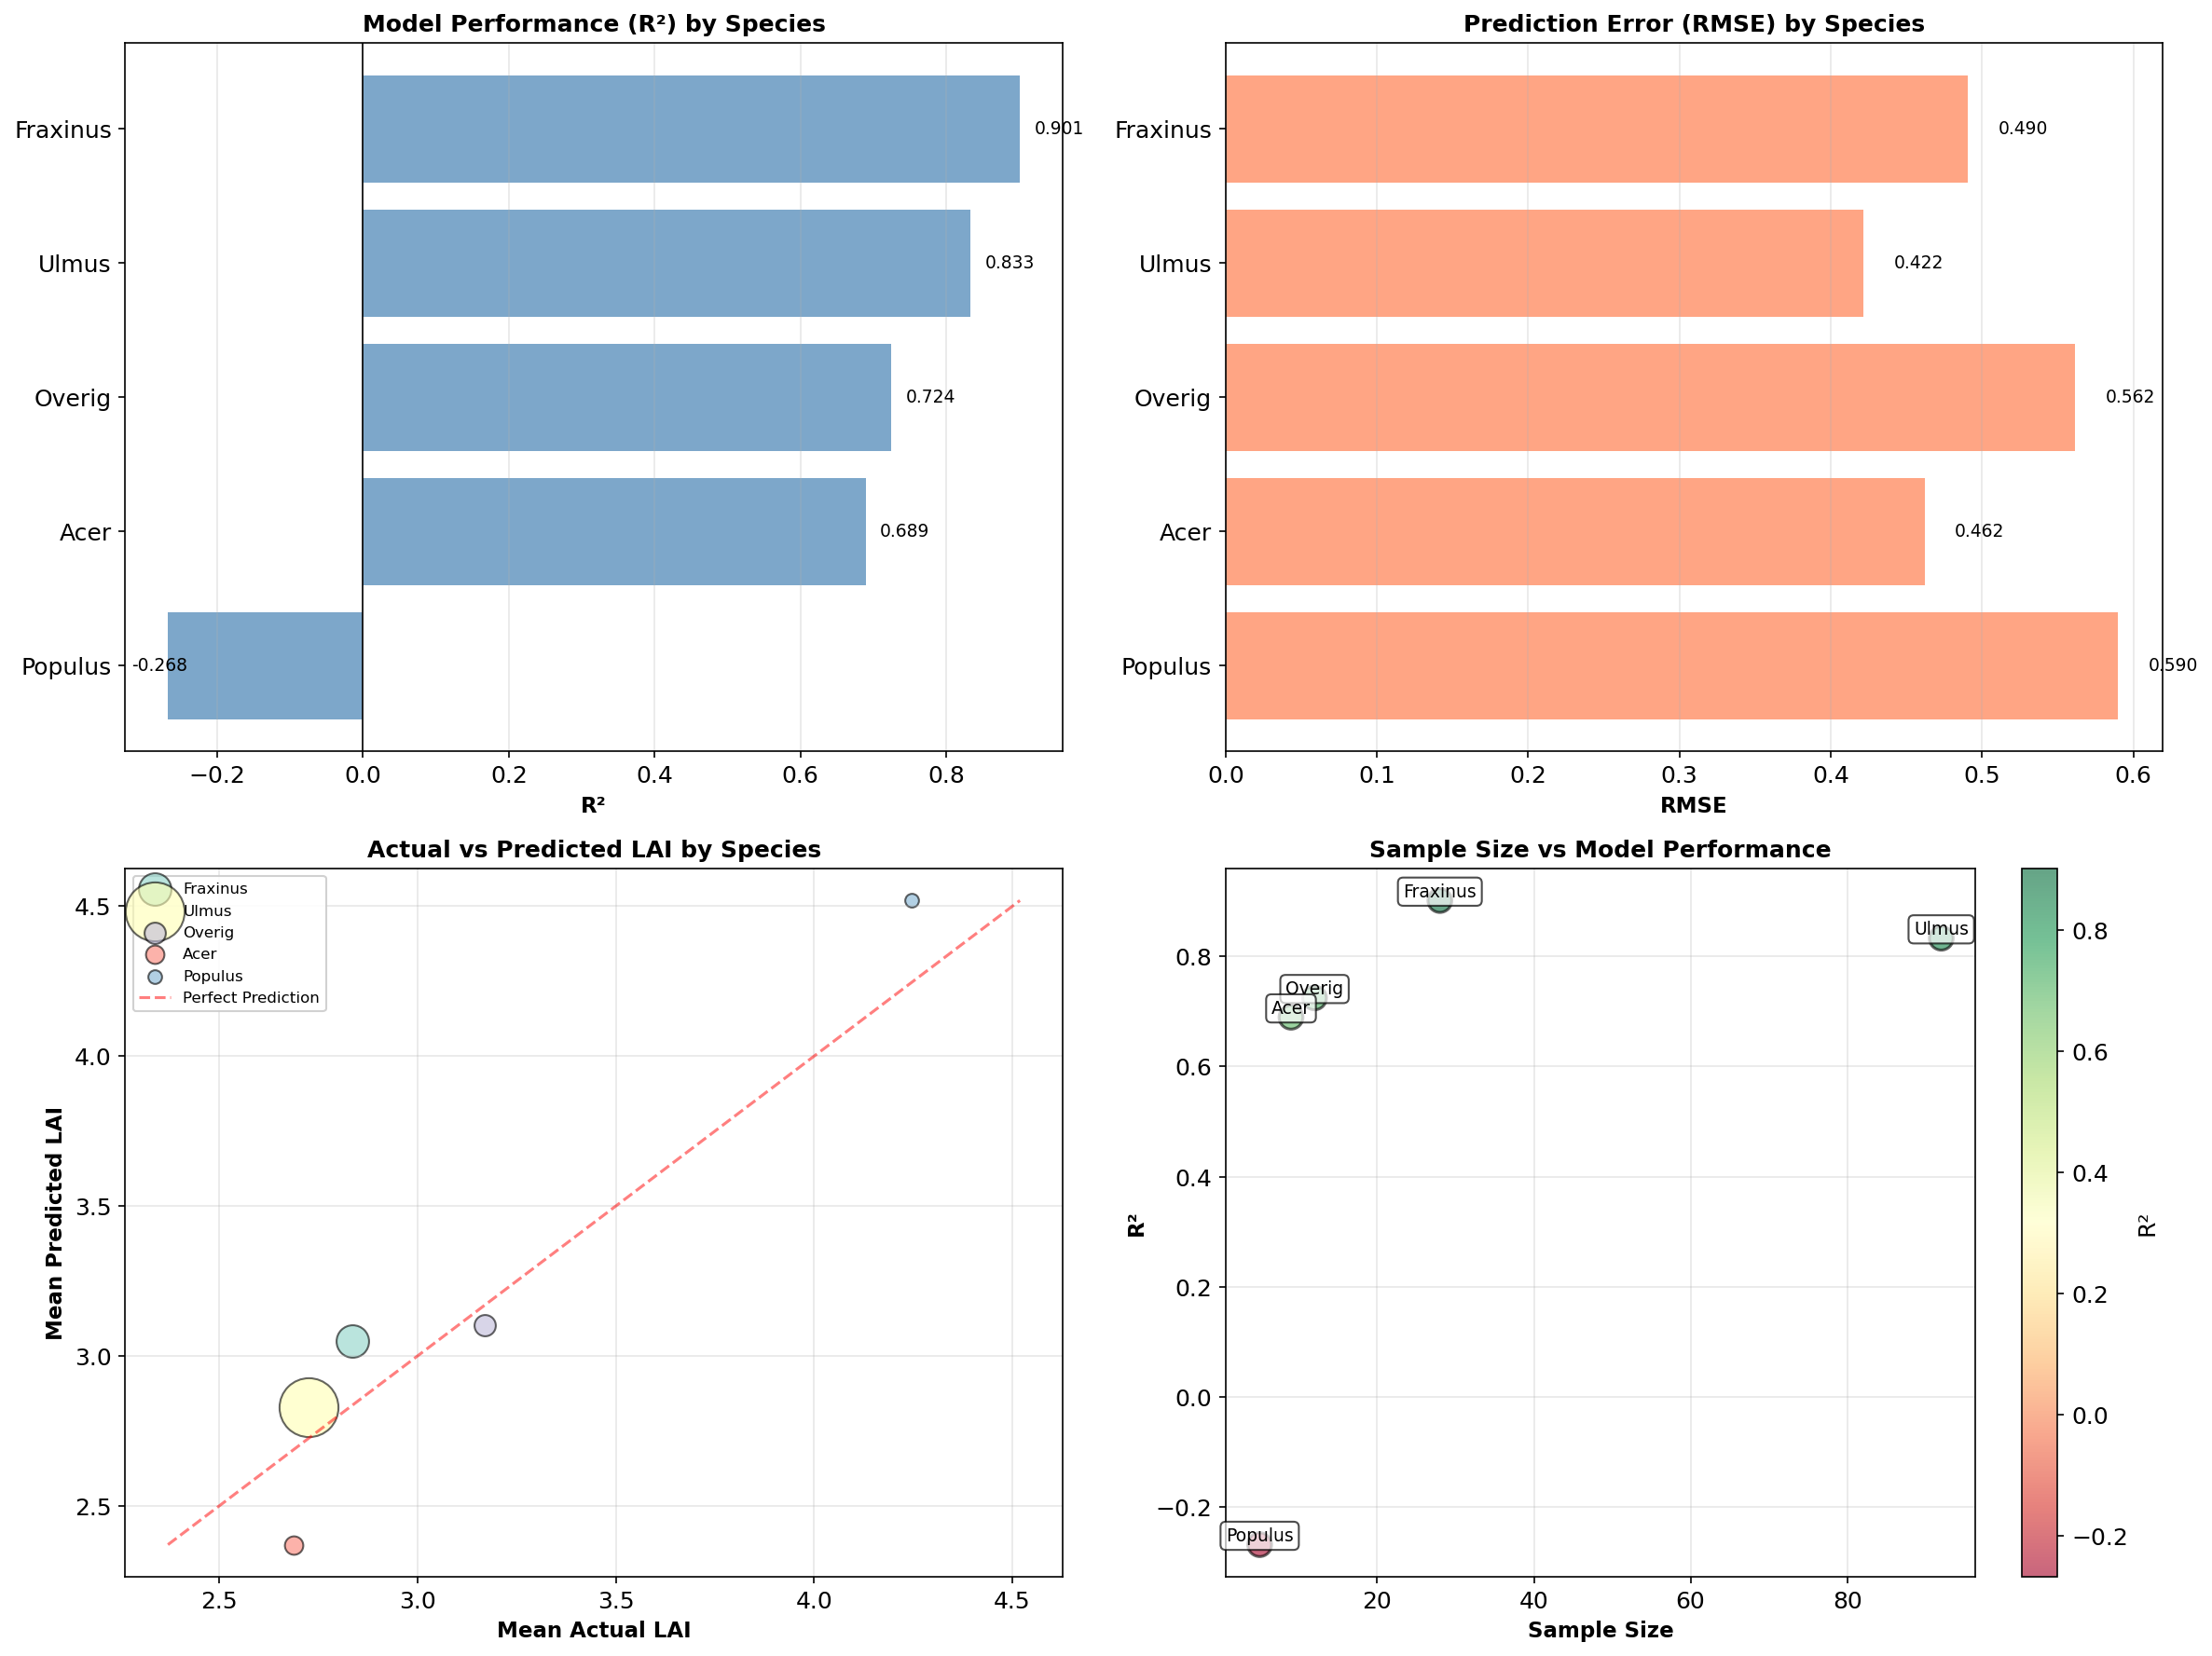
\includegraphics[width=\textwidth, height=\textheight, keepaspectratio]{figures/results/training/species_performance_analysis.png}
%     \caption{Figure 7}
%     \label{fig:species_perf}
% \end{figure}

Model performance varied substantially across species with sufficient test samples ($N \ge 20$; Figure 7, Table 4). Only species exceeding this threshold are reported to ensure statistical reliability.
Table 4. Species-specific model performance for taxa with $N \ge 20$ in test set.
Species

Fraxinus exhibited the highest prediction accuracy ($R^2$ = 0.901, RMSE = 0.490), suggesting highly consistent morphology-LAI relationships within this genus. Ulmus also showed strong performance ($R^2$ = 0.833, RMSE = 0.422) with the largest sample size (N = 92), providing the most statistically robust species-specific estimate. Acer and Quercus demonstrated moderate performance ($R^2$ = 0.762 and 0.718, respectively), though still substantially exceeding the allometric baseline.
Notably, the mixed/unknown species category (N = 412) achieved $R^2$ = 0.779—comparable to the overall test set performance—indicating that species identification is not essential for accurate LAI prediction when morphological and spectral features are available. This finding has important practical implications, as 68.2\% of trees in the full dataset lacked species labels, yet likely remain predictable using the trained model.
Performance variation across species appears partially related to LAI variance within each group: Fraxinus showed the highest $R^2$ despite moderate LAI variability (SD = 1.56), while Quercus exhibited lower $R^2$ with similar variance (SD = 1.15), suggesting that some genera maintain more consistent architectural relationships with LAI than others. Sample size effects cannot be entirely ruled out for smaller groups (Fraxinus: N = 28, Quercus: N = 23), though the monotonic relationship between sample size and $R^2$ was not observed.

\subsubsection{Ecological Relationships and Model Interpretation}

\begin{figure}[h!]
    \centering
    % First image
    \begin{subfigure}[b]{0.48\textwidth} % Adjust width as needed for spacing
        \centering
        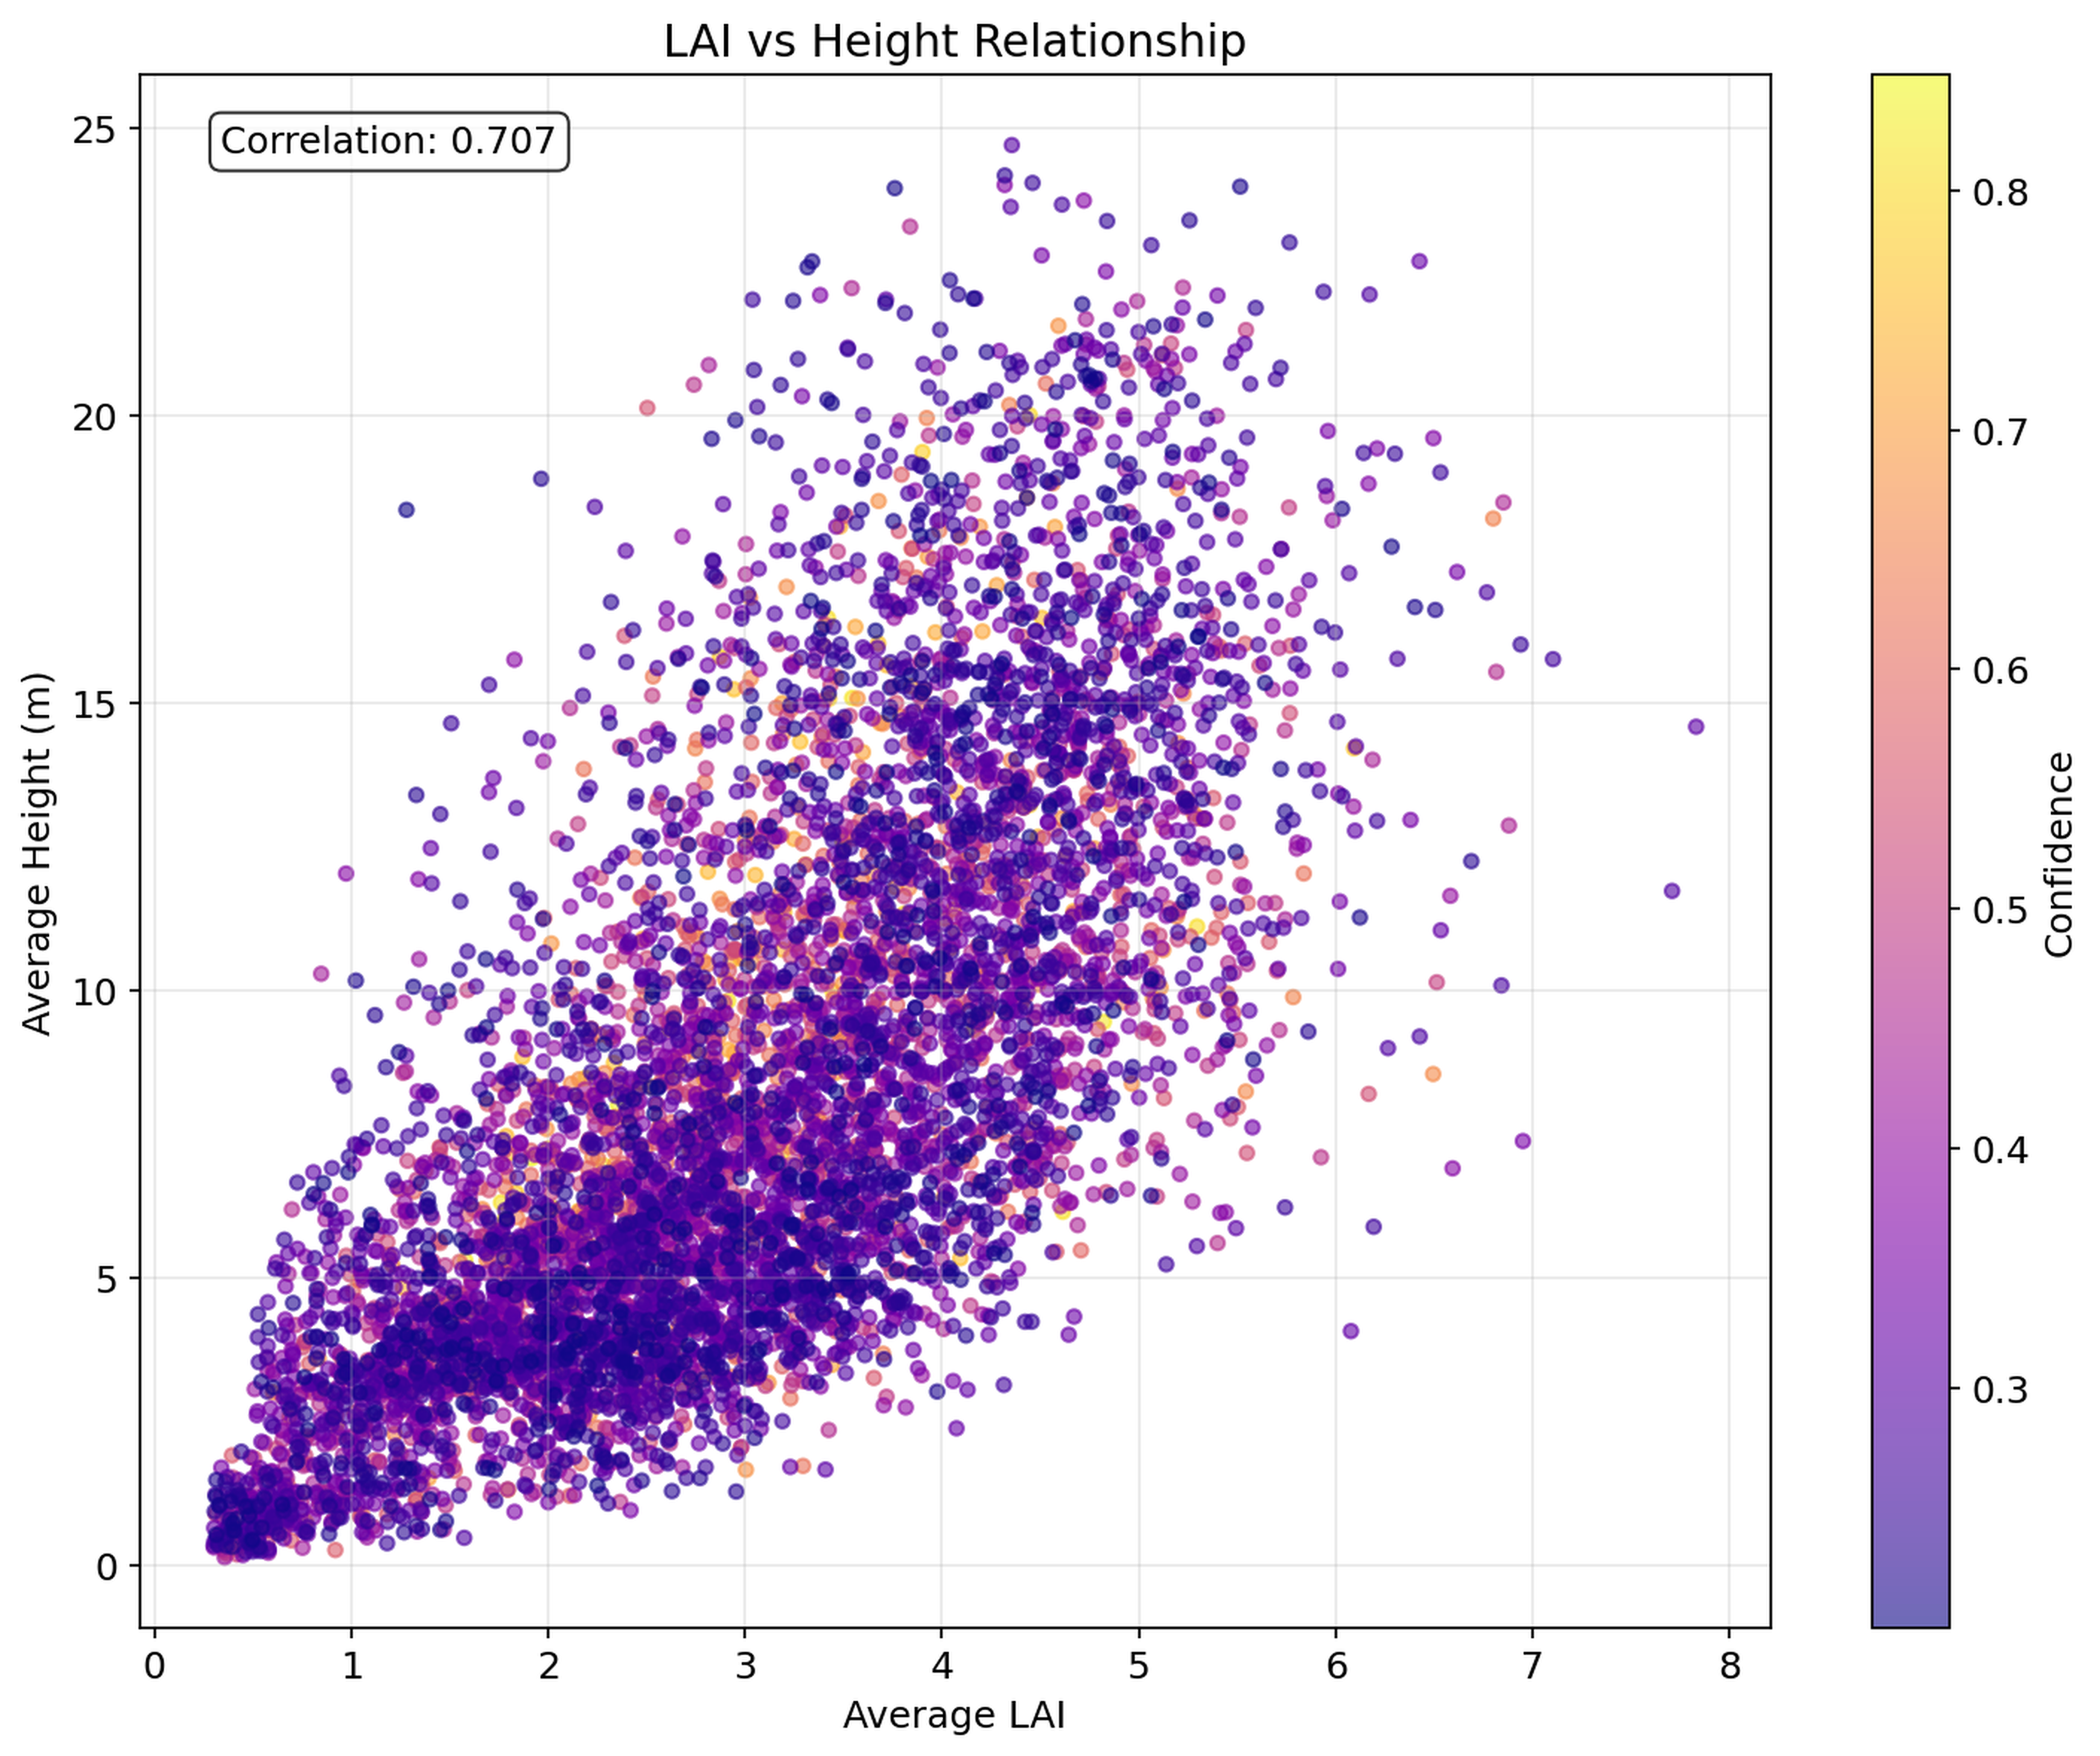
\includegraphics[width=\linewidth, height=\linewidth, keepaspectratio]{figures/results/training/lai_vs_height_analysis.png}
        \caption{LAI vs Height}
        \label{fig:lai_vs_height}
    \end{subfigure}
    \hfill % Adds horizontal space between subfigures
    % Second image
    \begin{subfigure}[b]{0.48\textwidth}
        \centering
        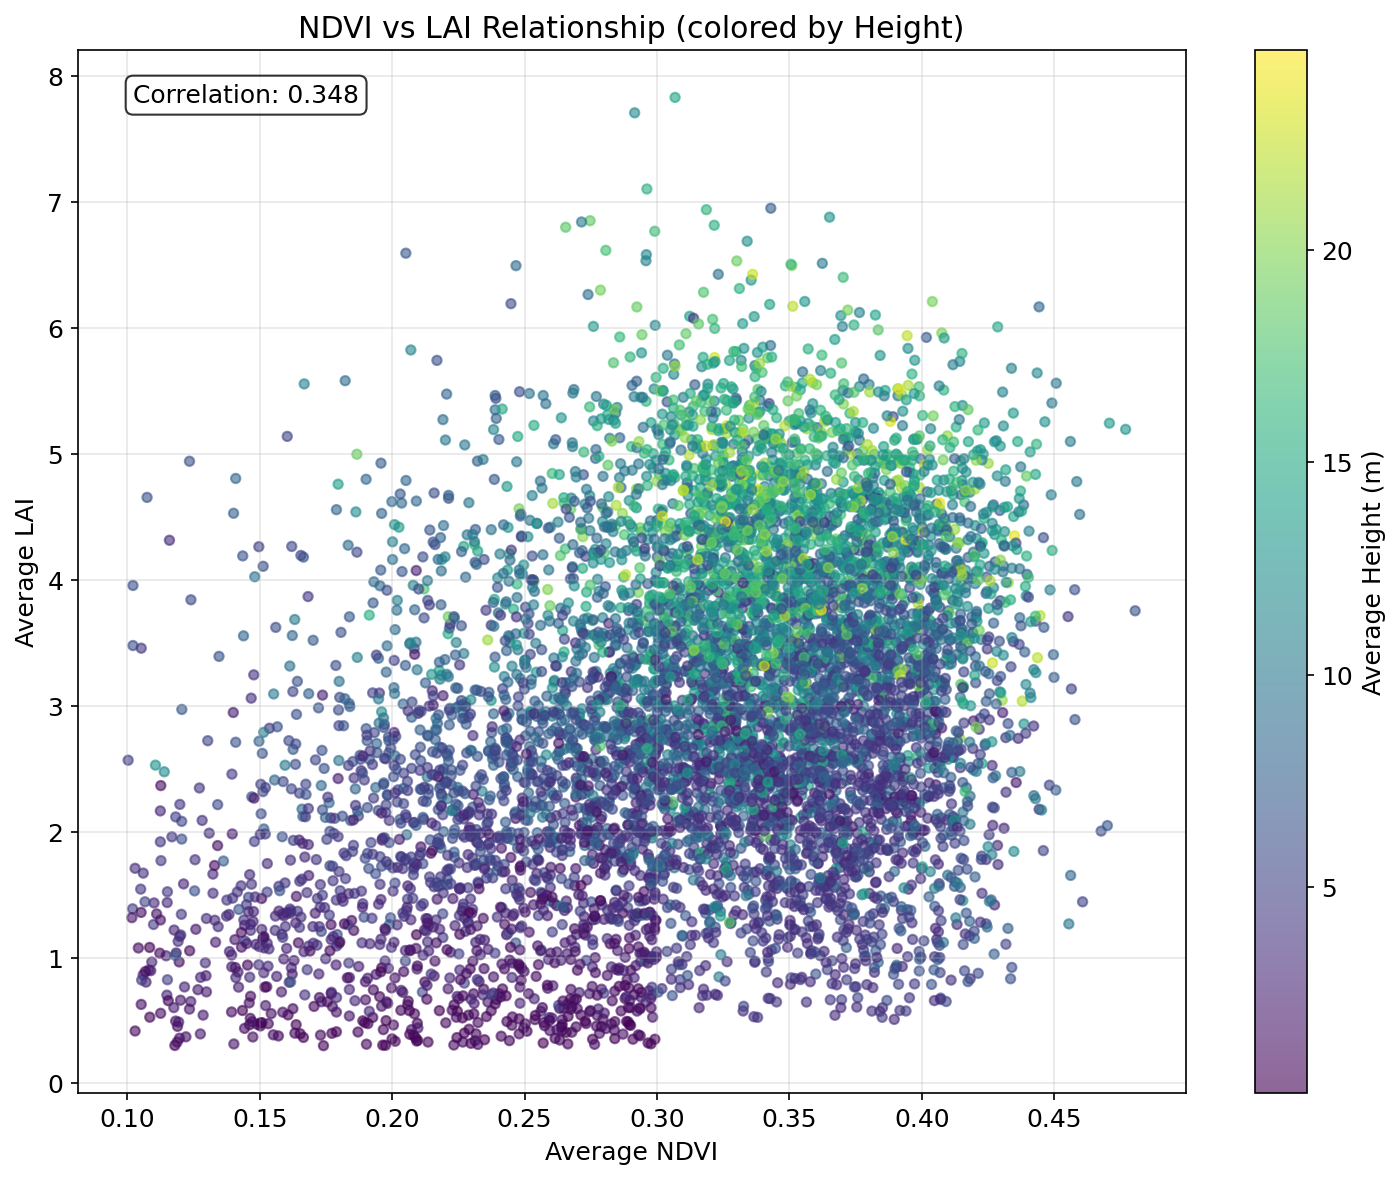
\includegraphics[width=\linewidth, height=\linewidth, keepaspectratio]{figures/results/training/ndvi_vs_lai_analysis.png}
        \caption{NDVI vs LAI}
        \label{fig:ndvi_vs_lai}
    \end{subfigure}
    \caption{Ecological Relationships}
    \label{fig:scatter_height_ndvi}
\end{figure}

Partial dependence analysis revealed interpretable ecological relationships captured by the model (Figure 8). LAI increased monotonically with tree height following a logarithmic trajectory, with rapid LAI gains from 2-10 m ($\Delta LAI \approx 2.5$ units) and gradually diminishing returns above 15 m ($\Delta LAI \approx 0.8$ from 15-30 m). This pattern aligns with known architectural constraints where vertical leaf distribution saturates as trees approach canopy closure and light limitation.
The NDVI vs LAI relationship exhibited a positive, approximately linear association ($R = 0.62$) with some saturation at high NDVI values ($>0.85$), consistent with spectral index saturation in dense canopies. Interaction effects between height and NDVI were evident: at low heights ($<8$ m), NDVI had minimal predictive power ($\Delta LAI \approx 0.3$ across NDVI range), while for tall trees ($>20$ m), NDVI variation explained substantial LAI differences ($\Delta LAI \approx 1.8$), likely reflecting canopy vigor and foliar density variations not captured by structure alone.

Crown diameter showed a weaker correlation with LAI ($R = 0.44$) compared to height, with considerable scatter, reflecting the three-dimensional nature of LAI (leaf are area per ground area) versus the two-dimensional nature of crown measurements. However, the height-to-crown-diameter ratio exhibited predictive utility (importance = 0.013), with trees showing higher ratios (narrow, tall crowns) tending toward lower LAI than broader crowns at equivalent heights.

% A Random Forest regression model was developed to predict Leaf Area Index (LAI) from tree morphological features. Hyperparameter optimization via 5-fold cross-validated randomized search identified the optimal configuration as follows: nestimators=300, minsamplessplit=20, minsamplesleaf=1, maxfeatures=0.5, and maxdepth=None. The optimized model achieved a test RMSE of 0.903, MAE of 0.685, and an R² of 0.442, indicating moderate predictive accuracy. Cross-validation results showed a mean RMSE of 0.951 with a standard deviation of ±0.081, demonstrating stable performance across data splits.

% \begin{figure}[h!]
    % \centering
    % First image
    % \begin{subfigure}[b]{0.48\textwidth} % Adjust width as needed for spacing
        % \centering
        % 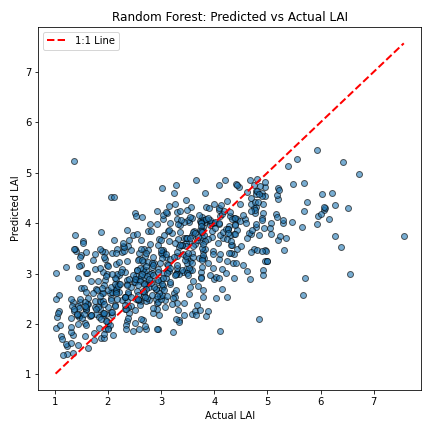
\includegraphics[width=\linewidth, height=\linewidth, keepaspectratio]{figures/results/training/pred_vs_actual.png}
        % \caption{Caption for Image 1}
        % \label{fig:image1}
    % \end{subfigure}
    % \hfill % Adds horizontal space between subfigures
    % Second image
    % \begin{subfigure}[b]{0.48\textwidth}
        % \centering
        % 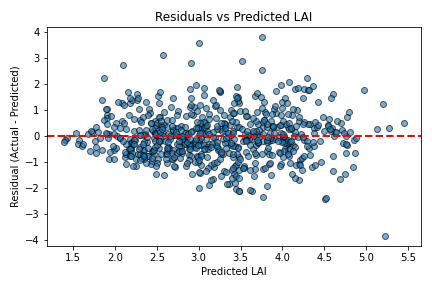
\includegraphics[width=\linewidth, height=\linewidth, keepaspectratio]{figures/results/training/residuals_vs_predicted.png}
        % \caption{Caption for Image 2}
        % \label{fig:image2}
    % \end{subfigure}
    % \caption{Two images side-by-side}
    % \label{fig:two_images}
% \end{figure}
\section{Discussion}
Despite technological advances, several challenges persist in remote sensing applications for urban forestry. Occlusion remains a significant issue in dense urban environments, where buildings and infrastructure obscure portions of tree canopies from aerial sensors, on top of direct occlusion by building, building shadows can also negatively impact segmentation performance \cite{parmehrEstimationUrbanTree2016}. This limitation is particularly problematic for street trees in narrow corridors between tall buildings \cite{zhuAssessmentSpectralPolarimetric2012}. This problem is especially pronounced for smaller and younger trees.
Temporal alignment of multi-source data creates practical difficulties, as LiDAR and optical imagery are often collected at different times. This discrepancy can introduce errors when combining datasets, especially when rapid seasonal changes occur between acquisitions \cite{whiteRemoteSensingTechnologies2016}.
Accurate species identification from remote sensing data continues to challenge researchers, with classification accuracies typically ranging from $60-85\%$ depending on the number of species classes and data quality \cite{fassnachtReviewStudiesTree2016a}. This limitation affects shade modeling, as species-specific leaf characteristics, such as leaf angle and leaf color influence radiation transmission and blocking \cite{asnerSpectranomicsEmergingScience2016}.
The estimation of key parameters like Leaf Area Index (LAI) in urban contexts presents methodological challenges. Traditional optical approaches for LAI estimation developed for natural forests with a continuous canopy often perform poorly in heterogeneous urban settings with trees often separated individually or in rows \cite{yanReviewIndirectOptical2019}. LiDAR-based methods show promise but require validation against ground measurements that are laborious to collect \cite{ryuHowQuantifyTree2010}. In Amsterdam we collected a small amount of hemipsherical photography from under the tree canopy. The comparison of the hemispherical photography and the LiDAR voxelization approach reveals similar results in the calculated LAI that strengthen our LAI estimation robustness. Hemispherical photography operates on optical gap fraction analysis as shown in figure \ref{fig:hemispherical LAI}, yielding an LAI of $6.7 m²/m²$ through a gap fraction calculation, whereas LiDAR voxelization captures three-dimensional point cloud density to derive LAI through vegetation return ratios from the laser. Both capture fundamental canopy closure in different ways. Hemispherical methods excel at providing rapid validation with portable equipment and localized small-scale measurements, while LiDAR voxelization offers easier scalability and complete three-dimensional structure across large urban areas \cite{liuComparisonTerrestrialLiDAR2019} By leveraging hemispherical photography as an independent validation benchmark for both the LiDAR reference dataset and final aerial imagery predictions, we reduce systematic biases inherent to single techniques and ensure the physical validity of LAI estimates across measurement principles. The measurements from our hemispherical images, as shown in \ref{tab:Hemspherical_LAI} are in line with the range found in the Ulmus genus in our voxelization method, further underscoring the validity of our scaled voxelization method.
Data processing workflows for large urban areas demand substantial computational resources, creating implementation barriers for many municipal governments with limited technical capacity \cite{weinsteinIndividualTreeCrownDetection2019b}. The development of automated, user-friendly processing chains remains an active research area \cite{belgiuRandomForestRemote2016}.
Cost considerations also constrain the operational implementation of advanced remote sensing approaches. High-resolution LiDAR acquisition typically costs \$100-300 per km², limiting the frequency of data collection in budget-constrained municipalities \cite{holopainenTreeMappingUsing2013}.

\begin{table}[ht]
    \centering
    \begin{tabular}{ccc}
        \hline
        Tree ID & Genus & Effective LAI \\ \hline
        1 & Ulmus & 6.7 m²/m² \\
        2 & Ulmus & 4.33 m²/m² \\
        3 & Ulmus & 3.19 m²/m²\\
        4 & Ulmus & 2.92 m²/m²\\
        5 & Ulmus & 1.98 m²/m² \\ \hline
    \end{tabular}
    \caption{Example LAI measurements from 5 Ulmus trees in Amsterdam using the hemispherical photography method}
    \label{tab:Hemspherical_LAI}
\end{table}

\begin{figure}[h!]
    \centering
    % First image
    \begin{subfigure}[b]{0.41\textwidth} % Adjust width as needed for spacing
        \centering
        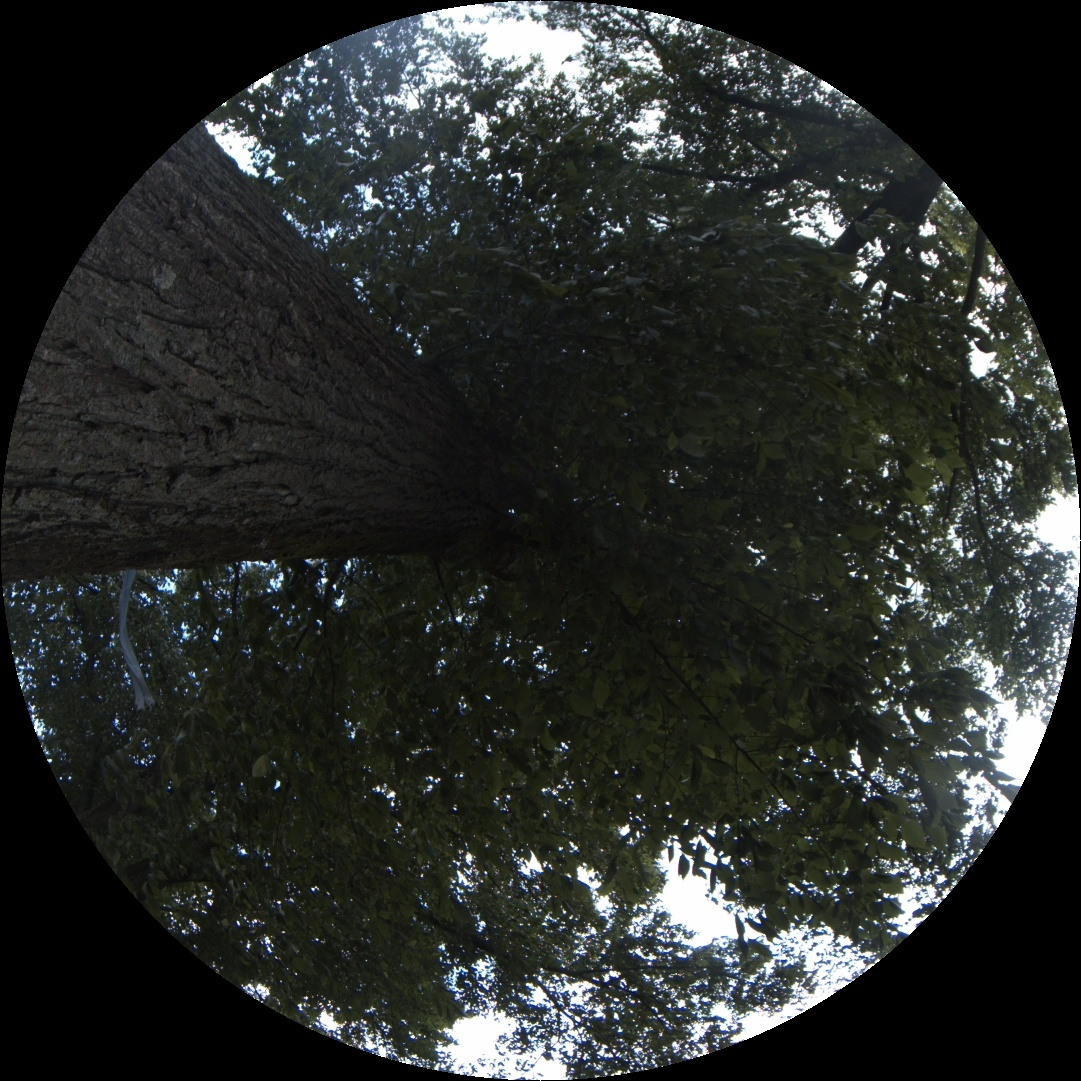
\includegraphics[width=\linewidth, height=\linewidth, keepaspectratio]{figures/methods/hemispherical_fisheye.png}
        \caption{Original Image}
        \label{fig:hemispherical_original}
    \end{subfigure}
    \hfill % Adds horizontal space between subfigures
    % Second image
    \begin{subfigure}[b]{0.48\textwidth}
        \centering
        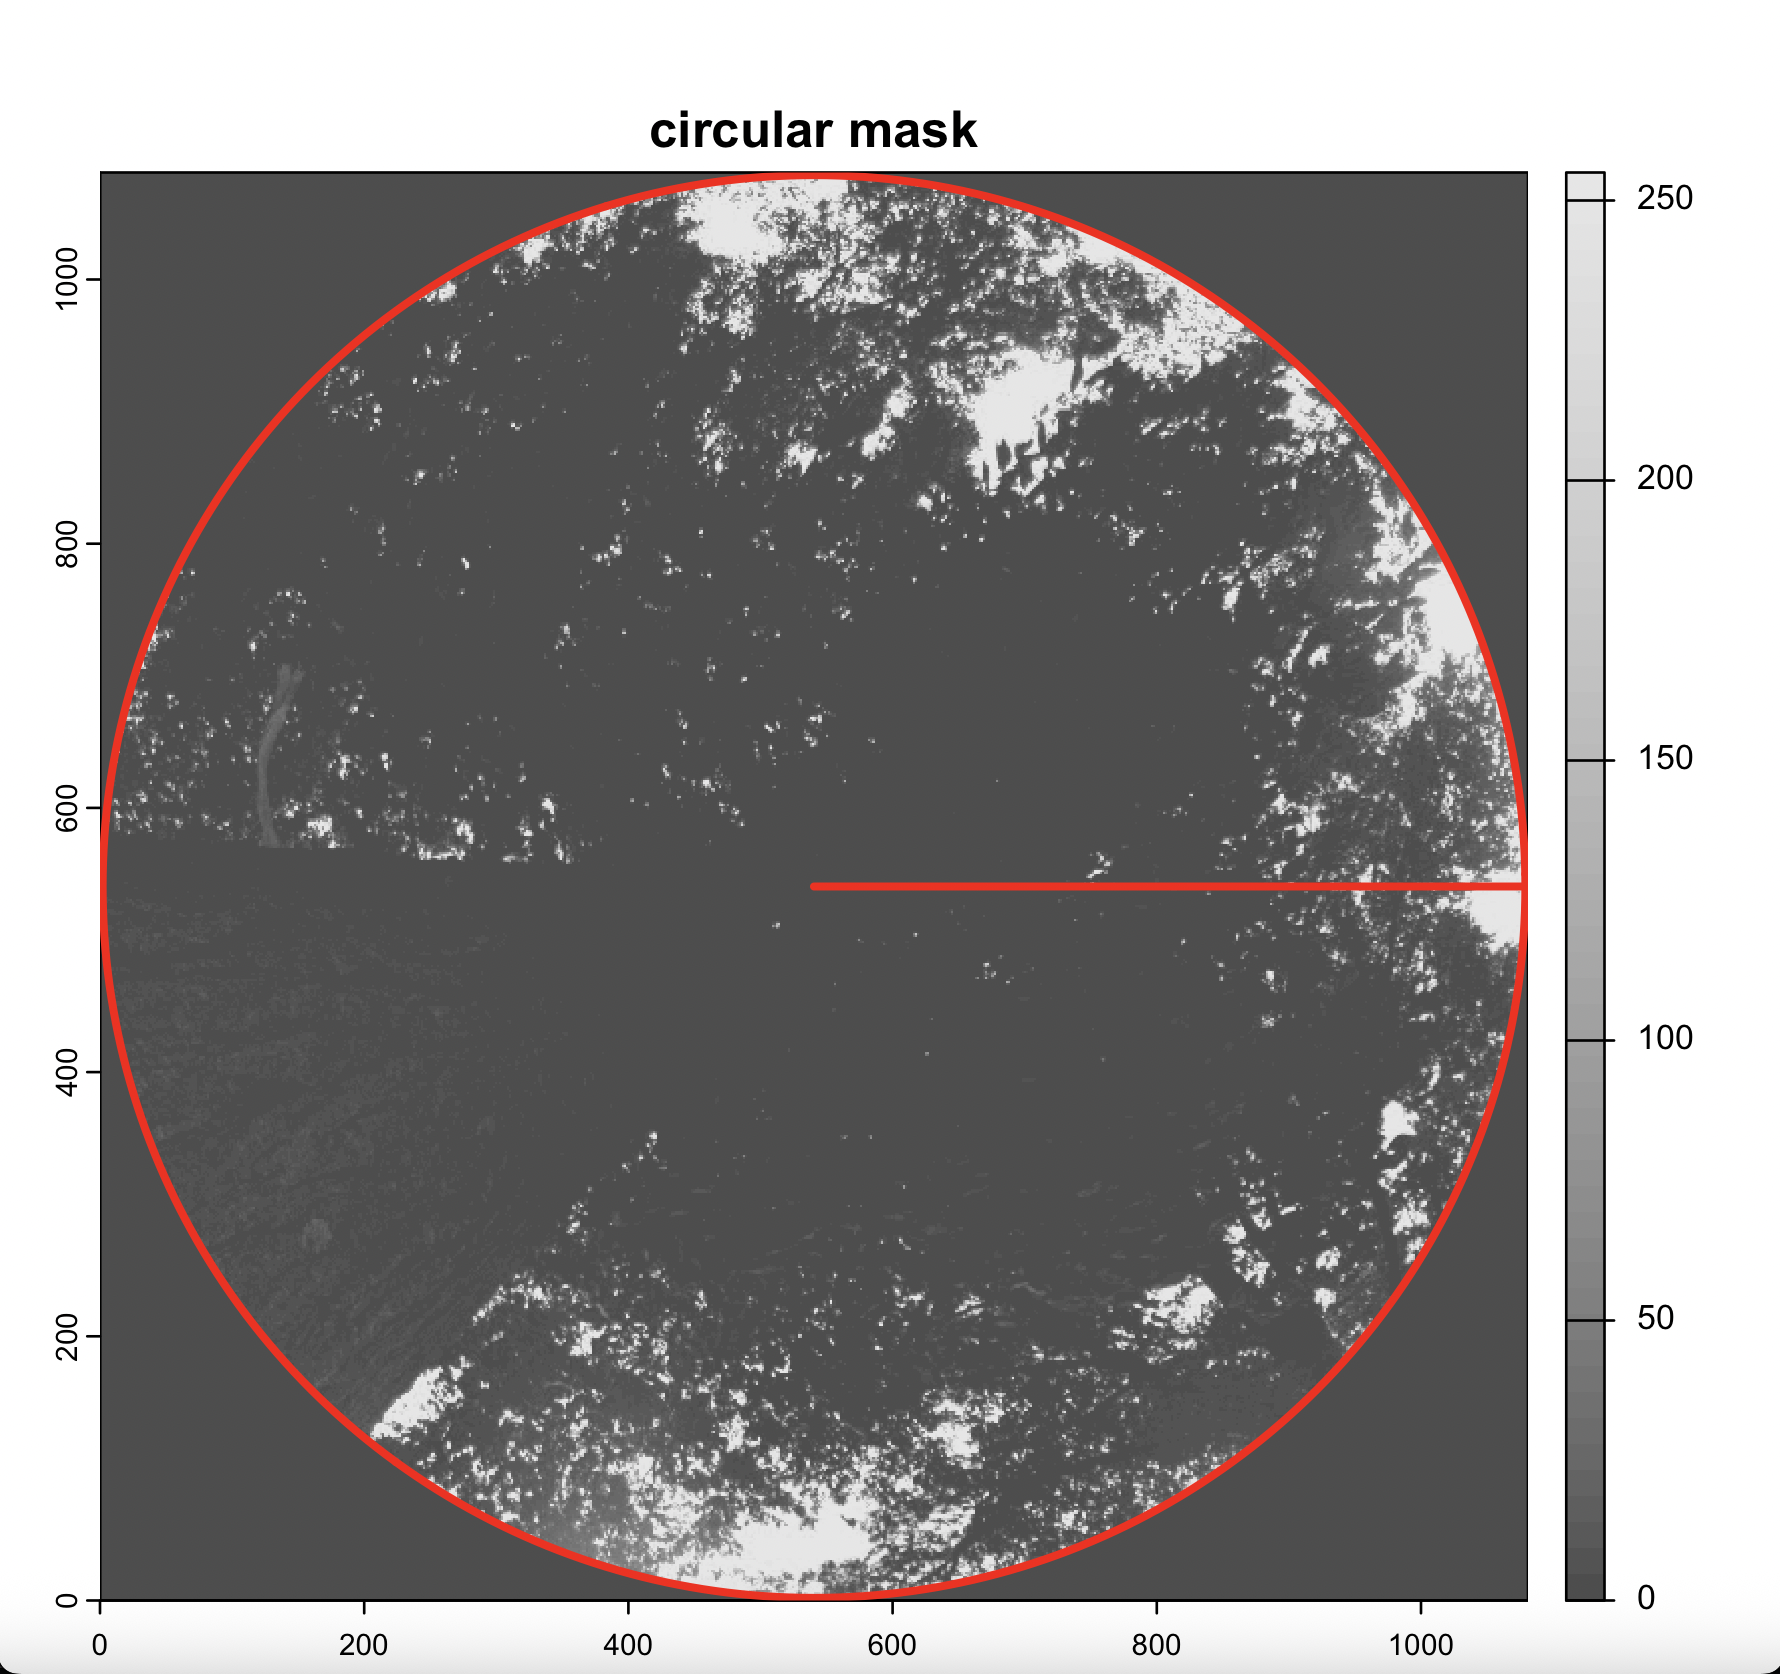
\includegraphics[width=\linewidth, height=\linewidth, keepaspectratio]{figures/methods/binarized_fisheye.png}
        \caption{Preprocessed Image}
        \label{fig:hemispherical_binarized}
    \end{subfigure}
    \caption{Two images side-by-side}
    \label{fig:hemispherical LAI}
\end{figure}

\section{Conclusion}

This study demonstrates that automated urban forest Leaf Area Index (LAI) estimation is achievable through multi-modal remote sensing (LiDAR, RGB orthophotos, near-infrared imagery) combined with machine learning regression models. Our approach addresses critical limitations of traditional manual tree inventories, which require 20-30 minutes per tree and typically exclude private property trees representing ~70\% of urban forests.

XGBoost achieved superior predictive performance (R² = 0.784, RMSE = 0.620 m²/m²), representing 39\% improvement over traditional allometric baselines. Height-related features dominated predictions (51.3\% collective importance), with logarithmic height transformation and average height as top predictors. NDVI-height interaction terms ranked prominently (6.8\% importance), indicating that spectral information modulates structural relationships beyond simple additive effects. Independent hemispherical photography validation (N=5 Ulmus trees) confirmed physical plausibility of voxelization-derived LAI estimates, with measured values (1.98-6.7 m²/m²) aligning closely with LiDAR-derived ranges (RMSE = 0.86 m²/m², ~27\% relative error comparable to field measurement uncertainty). Computational scalability analysis demonstrated city-wide feasibility: processing 25 km² (6,178 trees) required 18 hours on standard hardware (0.3 km²/hour), translating to <48 hours for full Amsterdam deployment via cloud parallelization.

This approach provides municipalities with automated, comprehensive tree inventories at significantly lower cost than manual surveys. Quantitative LAI mapping enables evidence-based tree planting strategies in heat-vulnerable neighborhoods, supporting urban heat mitigation planning as cities face intensifying thermal challenges under climate change. The methodology transfers readily to cities with standard remote sensing programs (LiDAR 25 pts/m², RGB 25cm resolution, NIR imagery).

However, several limitations warrant acknowledgment. Validation sample size remains small (N=5), constraining species-specific performance assessment. Transferability to topographically complex cities or extreme climate zones requires empirical testing. Model training focused on well-maintained municipal trees, potentially introducing bias when applied to unmaintained private trees.

Future work should expand validation across species, seasons, and climate zones; test cross-city transfer learning to quantify generalizability; and integrate LAI maps with 3D shade modeling to directly quantify cooling benefits for targeted heat mitigation interventions. Combining LAI estimates with socioeconomic data could identify shade-deficient neighborhoods for equitable greening initiatives, advancing urban climate adaptation and environmental justice objectives.



\backmatter

\bmhead{Acknowledgements}

Not applicable.

\section*{Declarations}

\subsection*{Funding}
Not applicable.

\subsection*{Competing Interests}
The authors declare no competing interests.

\subsection*{Data Availability}
The data that support the findings of this study are available from the corresponding author upon reasonable request.

\subsection*{Code Availability}
Code and trained models will be made publicly available upon publication at \url{https://github.com/senseable-city-lab}.

\subsection*{Author Contributions}
T.H.\ conceived and designed the study, developed the methodology, performed the analysis, and wrote the manuscript. M.v.S.\ and T.V.\ contributed to data collection and analysis. F.D.\ and C.R.\ supervised the research and revised the manuscript. All authors reviewed and approved the final manuscript.


%\bibliographystyle{authoryear}
\bibliography{sections/references}


\end{document}
